%% 
%% Copyright 2019-2020 Elsevier Ltd
%% 
%% This file is part of the 'CAS Bundle'.
%% --------------------------------------
%% 
%% It may be distributed under the conditions of the LaTeX Project Public
%% License, either version 1.2 of this license or (at your option) any
%% later version. The latest version of this license is in
%%    http://www.latex-project.org/lppl.txt
%% and version 1.2 or later is part of all distributions of LaTeX
%% version 1999/12/01 or later.
%% 
%% The list of all files belonging to the 'CAS Bundle' is
%% given in the file `manifest.txt'.
%% 
%% Template article for cas-dc documentclass for 
%% double column output.

%\documentclass[a4paper,fleqn,longmktitle]{cas-dc}
\documentclass[a4paper,fleqn]{cas-dc}

% \usepackage[authoryear,longnamesfirst]{natbib}
%\usepackage[authoryear]{natbib}
\usepackage[numbers,sort&compress]{natbib}

\usepackage{algorithm}
\usepackage{algpseudocode}
\renewcommand{\algorithmicrequire}{\textbf{Input:}}  % Use Input in the format of Algorithm  
\renewcommand{\algorithmicensure}{\textbf{Output:}} % Use Output in the format of Algorithm 

\usepackage{threeparttable}%表格下面加标注
\usepackage{algpseudocode}
\usepackage{threeparttable}%表格下面加标注
\usepackage{rotating}

% Attempt to fix the \pdf@box issue: load graphicx with pdftex driver and color
%\usepackage[pdftex]{graphicx}
%\usepackage{color}

% Now load hyperref (also with pdftex driver to be consistent? Actually, hyperref will use the driver automatically)
%\usepackage{hyperref}
\usepackage{float}
\usepackage{array, longtable, tabularx}
%\usepackage{caption}

\usepackage{cleveref} % 确保 cleveref 已加载
\crefname{figure}{}{}% 设置 \cref 对 figure 的引用格式为空(只留编号)
\Crefname{figure}{}{}% 设置 \Cref 对 figure 的引用格式为空(只留编号)
\crefname{table}{}{}% 设置 \cref 对 figure 的引用格式为空(只留编号)
\Crefname{table}{}{}% 设置 \Cref 对 figure 的引用格式为空(只留编号)
\crefname{section}{}{}% 设置 \cref 对 figure 的引用格式为空(只留编号)
\Crefname{section}{}{}% 设置 \Cref 对 figure 的引用格式为空(只留编号)
\usepackage{float}
\usepackage{array, longtable, tabularx}

\sloppy
%%%Author definitions
\def\tsc#1{\csdef{#1}{\textsc{\lowercase{#1}}\xspace}}
\tsc{WGM}
\tsc{QE}
\tsc{EP}
\tsc{PMS}
\tsc{BEC}
\tsc{DE}
%%% 

\begin{document}
\let\ref\Cref 		
\let\eqref\Cref 	
\let\autoref\Cref 	
\let\WriteBookmarks\relax
\def\floatpagepagefraction{1}
\def\textpagefraction{.001}
\shorttitle{Journal of Engineering Research xx (20xx) xxxxxx}
\shortauthors{Author 1 and N.S. Ahmad}
\footmarks{\url{https://doi.org/10.1016/j.jer.20xx.xx.xxx}\\
    0952-1976/\begingroup\tiny{©}\endgroup~2025 Elsevier B.V.\\
    This is an open access article under the CC BY-NC-ND license (\url{http://creativecommons.org/licenses/by-nc-nd/4.0/}).
}


% \bookmark[named = FirstPage]{A Comprehensive Survey on UWB-Based NLOS Identification and Ranging Error Mitigation Using CIR Features and Raw Sequences} % Title bookmark used in the pdf
%**************** If the title is short, stay on the first line use [mode = short_title] otherwise ******************
%***************************************** use [mode = title] below ***************************************
\title [mode = title]{Advances in Autonomous Fruit-Picking Robots: Methodologies, Technologies, and Challenges}    

% Title mark notes if desired
%\tnotemark[1,2]

%\tnotetext[1]{This document is the results of the research
%   project funded by the National Science Foundation.}

%\tnotetext[2]{The second title footnote which is a longer text matter
%   to fill through the whole text width and overflow into
%   another line in the footnotes area of the first page.}

\author[1,2]{Zhihao Zhao}[type=author, 
                        auid=000,bioid=1,
                        ]
% \ead{wangshoude@usm.my}
\credit{Conceptualization of this study, Methodology}

\address[1]{School of Electrical and Electronic Engineering, Universiti Sains Malaysia, 14300 Nibong Tebal, Penang, Malaysia}

\author[3]{Yanxiang Zhao}
\author[1]{Nur Syazreen Ahmad}[type=author, 
                        auid=001,bioid=2,
                        orcid=0000-0001-7511-2910
                        ]
%\fnmark[1]
\cormark[1]
% \ead{syazreen@usm.my}
\credit{Data curation, Writing-Original draft preparation}

\address[2]{YanTai Engineering and Technology College, 264006 YanTai, Shandong, China}
\address[3]{Central South University, Changsha, Hunan, 410083, China}
% \author[1,3]{CV Radhakrishnan}[type=editor, 
%                         auid=000,bioid=1,
%                         prefix=Sir,
%                         %role=Researcher,
%                         %orcid=0000-0001-7511-2910
%                         ]
% \cormark[1]
% %\fnmark[1]								% URL related footnote marking
% \ead{cvr_1@tug.org.in}
% %\ead[url]{www.cvr.cc, cvr@sayahna.org} % Author URL 

% \credit{Conceptualization of this study, Methodology, Software}

% \address[1]{Elsevier B.V., Radarweg 29, 1043 NX Amsterdam, The Netherlands}

% \author[2,3]{Han Theh Thanh}[style=chinese]

% \author[2,3]{CV Rajagopal}[
%    %role=Co-ordinator,
%    suffix=Jr,
%    ]
% %\fnmark[2]								% URL related footnote marking
% \ead{cvr3@sayahna.org}
% %\ead[URL]{www.sayahna.org}				% Author URL

% \credit{Data curation, Writing - Original draft preparation}

% \address[2]{Sayahna Foundation, Jagathy, Trivandrum 695014, India}

% \author
% [1,3]
% {Rishi T.} % If the author's name hits "Check for updates" button, use \\ at the break point of his/her name like {\\Rishi T.} or {First Middle\\ Lastname}
% % NOTE: Compile first without \\ then the proper separation again afterwards !!! (Not doing so, results unwanted footnote and Credit authorship contribution at the very end with \credit command if used.)
% \cormark[2]
% %\fnmark[1,3]							% URL related footnote marking
% \ead{rishi@stmdocs.in}
% %\ead[URL]{www.stmdocs.in}				% Author URL

% \address[3]{STM Document Engineering Pvt Ltd., Mepukada,
%     Malayinkil, Trivandrum 695571, India}

% \author[4]{ \\Salih Baris Ozturk} % Author's name hits "Check for updates" button, \\ is used at the break point of his name. If \\ is desired at the beginning of the name, place a space just before the \\ as in the above example.
% % NOTE: Compile first without \\ and the space, then the proper separation again afterwards !!! (Not doing so, results unwanted footnote and Credit authorship contribution at the very end with \credit command if used.)
% %\cormark[1]
% \ead{ozturksb@itu.edu.tr}

% \address[4]{Istanbul Technical University, Department of Electrical Engineering,
% 	Maslak, Istanbul 34469, Turkey}

\credit{Modification for the final layout}

\cortext[1]{Corresponding author.}
% \cortext[cor2]{Principal corresponding author.}
% \fntext[1]{E-mail address: \href{mailto:syazreen@usm.my}{syazreen@usm.my} (N.S. Ahmad).}
%\fntext[fn2]{Another author footnote, this is a very long footnote and
%  it should be a really long footnote. But this footnote is not yet
%  sufficiently long enough to make two lines of footnote text.}

%\nonumnote{This note has no numbers. In this work we demonstrate $a_b$
%  the formation Y\_1 of a new type of polariton on the interface
%  between a cuprous oxide slab and a polystyrene micro-sphere placed
%  on the slab. The evanescent field of the resonant whispering 
%  gallery mode (\WGM) of the micro sphere has a substantial 
%  gradient, and therefore effectively couples with the
%  quadrupole $1S$ excitons in cuprous oxide.}

\nonumnote{E-mail address: \href{mailto:syazreen@usm.my}{syazreen@usm.my} (N.S. Ahmad).}

\begin{abstract} 
The advent of autonomous fruit-picking robots has precipitated a paradigm shift in contemporary agriculture, with the potential to address the prevailing labour shortage and enhance harvesting efficiency. This review comprehensively surveys recent progress in fruit-picking robotics, focusing on vision-based detection, learning-based strategies, arm motion planning, and collision avoidance. Employing a Preferred Reporting Items for Systematic Reviews and Meta-Analyses (PRISMA)-based systematic methodology, over 130 influential studies from 2015–2024 were analysed. Recent advances in vision-based detection, including multi-sensor fusion and 3D data acquisition, have enhanced robots' ability to localise and identify fruits under complex agricultural conditions. 
Deep learning (DL) models, such as Regions with Convolutional Neural Networks (R-CNN) and You Only Look Once (YOLO) series, have demonstrated efficacy in enhancing real-time detection performance, particularly under occlusion and variable lighting.
%The efficacy of deep learning (DL) models, such as the Regions with Convolutional Neural Networks (R-CNN) and You Only Look Once (YOLO) series, has been demonstrated in enhancing real-time detection performance, particularly in scenarios where there is occlusion and variable lighting. 
It is evident that learning-based approaches, including transfer learning and reinforcement learning (e.g., Deep Deterministic Policy Gradient (DDPG)), have enhanced the generalisation capabilities and optimised the robotic arm motion planning for collision-free harvesting. Innovative path-planning algorithms and robust control strategies further enable autonomous robots to navigate unstructured environments and compensate for real-time disturbances, increasing system reliability. 
Despite these advances, challenges remain in multi-source data integration and delicate handling. This survey provides a comprehensive evaluation of technological advancements, identifies research gaps in scalability and deployment, and proposes future directions to guide research and accelerate commercial adoption.
%Notwithstanding these advances, challenges persist in guaranteeing precise multi-source data integration, delicate fruit handling, and robust operation across diverse and unpredictable environments. The paper highlights trends towards the integration of the Internet of Things (IoT), advanced sensors, and machine learning (ML). It identifies research gaps in scalability and real-world deployment, and proposes future research directions. This survey provides a comprehensive and critical evaluation of technological advancements and ongoing challenges in the field of autonomous fruit-picking robotics. The primary objective of the survey is to provide a foundation for guiding future research and accelerating the commercial adoption of these transformative systems.

\end{abstract}

% If any graphical abstract is needed
%\begin{graphicalabstract}
%\includegraphics{figs/grabs.pdf}
%\end{graphicalabstract}

% If any highlights is needed above the cover page
%\begin{highlights}
%\item Research highlights item 1
%\item Research highlights item 2
%\item Research highlights item 3
%\end{highlights}

% Article history - Should only be set by an editor
\received {xx Month 20xx}
\revised {xx Month 20xx}
\accepted {xx Month 20xx}
\online {xx Month 20xx}

\begin{keywords}
 Autonomous Fruit-Picking Robots,
Regions with Convolutional Neural Networks (R-CNN),
You Only Look Once (YOLO),
Motion Planning,
Transfer Learning.
\end{keywords}

\maketitle

\section{Introduction}
The advent of autonomous fruit-picking robots represents a significant evolution in agricultural technology, driven by the need to address labor shortages, escalating costs, and the demand for enhanced efficiency in fruit production. 
%Rapid advancements in robotics and artificial intelligence have catalyzed substantial interest in developing fruit-picking robots. These robots promise to revolutionize agricultural practices by automating labor-intensive fruit harvesting. Fruit-picking robots are autonomous systems engineered to identify, locate, and harvest fruits from various trees and plants. 
These systems leverage advanced technologies, including computer vision, machine learning (ML), robotics, and the Internet of Things (IoT), to operate efficiently in diverse agricultural environments, handle fruits delicately, and complement human labor.
%These systems leverage a suite of advanced technologies, including computer vision, machine learning (ML), robotics, and Internet of Things (IoT). The aim is to create robots that can operate efficiently in various agricultural environments, handle fruits delicately to avoid damage, and work alongside human labor to enhance productivity. 
%like Figure~\ref{fig:fruit_picking_robot_overview}.
Recent advancements in deep learning (DL) and sensor fusion have facilitated the development of sophisticated perception and motion control mechanisms, enabling robots to detect, localize, and harvest fruits with increasing precision. Figure ~\ref{fig:struct} illustrates the general architecture of an autonomous fruit-picking robot, highlighting key components such as visual sensors for detection, manipulator arms for grasping, and navigation systems for mobility. This progress has been particularly evident in addressing challenges like occlusion, variable lighting, and unstructured orchards.

Existing literature reviews have laid the groundwork for understanding advancements in autonomous fruit-picking technologies as summarized in Table~\ref{tab:survey_summary}. These recent surveys, all published since 2021, have collectively advanced the field by addressing various aspects of robotic systems, though they often exhibit limitations in scope and integration.
For instance, Hou et al. \cite{hou2023overview} focused on the integration of deep learning (DL) with multi-sensor vision systems, emphasizing perception sensors and machine vision to enhance fruit detection in unstructured environments. While this work provided valuable insights into AI-driven fusion and trends in field robustness, it overlooked broader system integration and actuation mechanisms. Similarly, Navas et al. \cite{navas2021soft} specialized in soft and bionic gripper designs, advancing understanding of adaptive handling for delicate fruits from a mechanical perspective, but neglected upstream components like perception or downstream integration, resulting in a siloed approach.
In contrast, more comprehensive reviews such as those by Zhang et al. \cite{zhang2024automatic} and Mingyou et al. \cite{mingyou2024orchard} adopted end-to-end perspectives. Zhang et al. covered machine vision, motion planning, end-effectors, mechanical automation, system integration, and field adaptation, notably including real-time control via IoT/5G and economic feasibility assessments for practical deployment. Mingyou et al. extended this by addressing multi-robot coordination and large-scale perception in expansive orchard settings, innovating with robust mapping and cooperative robotics trends. These works excelled in promoting holistic views but were sometimes constrained by their emphasis on specific deployment scenarios, such as large-scale orchards, potentially limiting applicability to smaller or diverse crop types.
Other surveys, including Zhou et al. \cite{zhou2022intelligent} and Rajendran et al. \cite{rajendran2024towards}, emphasized modular architectures and precision control. Zhou et al. explored machine vision, motion planning, and field adaptation, highlighting vision-driven precision and scalable designs for orchard autonomy, though without delving into mechanical details or cooperative elements. Rajendran et al. integrated perception sensors, machine vision, end-effectors, and field adaptation to discuss dexterous control and selective harvesting synergies, improving real-field reliability, yet their scope was somewhat narrow, focusing on targeted operations without broader multi-crop generalizations. Collectively, these surveys advanced the field by identifying key performance indicators, such as detection accuracy and adaptability metrics, but their fragmentation—often isolating components like perception from action or constraining to specific fruits (e.g., apples or citrus)—left gaps in fully end-to-end frameworks that encompass diverse agricultural contexts.
%This section reviews the primary contributions of some key surveys, highlighting their scopes and insights, followed by a discussion of their collective limitations, which motivate the innovations in this paper.
%Hou et al. \cite{hou2023overview}  focused on the integration of deep learning (DL) with multi-sensor vision systems. Their survey emphasized perception sensors and machine vision, detailing how AI-driven fusion enhances fruit detection in unstructured environments. This work highlighted trends in field robustness but overlooked broader system integration and actuation mechanisms.
%Zhang et al. \cite{zhang2024automatic}  provided an end-to-end perspective on automation chains, covering machine vision, motion planning, end-effectors, mechanical automation, system integration, and field adaptation. A notable contribution was the inclusion of real-time control via IoT/5G and economic feasibility assessments, offering a holistic view of practical deployment.
%Navas et al. \cite{navas2021soft} specialized in soft and bionic gripper designs, concentrating exclusively on end-effectors. Their analysis advanced understanding of adaptive handling for delicate fruits, drawing from mechanical perspectives, though it neglected upstream components like perception or downstream integration.
%Zhou et al. \cite{zhou2022intelligent} explored modular architectures, with emphasis on machine vision, motion planning, and field adaptation. Key insights included vision-driven precision and robot autonomy in orchards, promoting scalable designs that enhance adaptability without delving into mechanical details or cooperative elements.
%Mingyou et al. \cite{mingyou2024orchard}  addressed multi-robot coordination and large-scale perception, covering machine vision, motion planning, mechanical automation, system integration, and field adaptation. This survey innovated by focusing on robust mapping and execution in expansive orchard settings, incorporating cooperative robotics trends.
%Rajendran et al. \cite{rajendran2024towards} integrated perception sensors, machine vision, end-effectors, and field adaptation to discuss precision and dexterous control. Their contribution centered on selective harvesting synergies, improving real-field reliability for targeted operations.

%While these surveys collectively advance the discourse on fruit-picking robotics, several limitations persist that hinder a fully integrated and forward-looking understanding of the field. First, many exhibit a narrow temporal scope or outdated coverage; 
%While prior surveys have advanced the field as summarized in Table ~\ref{tab:survey_summary}, they exhibit limitations that our work addresses. 
%For instance, many have a narrow temporal scope, focusing predominantly on literature before 2020 and overlooking recent breakthroughs in DL models like YOLOv8.
% Zhou et al. and Navas et al. end in 2021, missing pivotal post-2022 developments in AI and multimodal sensing. Hou et al. and Rajendran et al. extend to 2022-2023 but underexplore emerging trends like unified benchmarking or cost-feasibility analyses, which are critical for industrial translation.
%A deeper issue is the siloed focus on specific subsystems: Navas et al. isolates end-effectors without linking to perception-action loops, while Hou et al. prioritizes vision but ignores motion planning and mechanical automation. This fragmentation leads to incomplete end-to-end frameworks, as seen in the absence of system integration in several works (e.g., Hou, Navas, Zhou, and Rajendran). Moreover, cooperative robotics and benchmarking are inconsistently addressed. Mingyou et al. touches on multi-robot aspects, but others largely omit them, resulting in a lack of standardized evaluation metrics for cross-study comparisons. Zhang et al. makes strides in economic feasibility, yet this is not uniformly integrated across surveys, often overlooking practical barriers like deployment costs and scalability in diverse agricultural contexts.
% Additionally, several adopt a siloed approach, emphasizing isolated aspects such as detection or grasping without integrating them into a cohesive end-to-end framework. This fragmentation underscores gaps in holistic analyses, which we bridge through a 'perception-action' approach that encompasses multi-sensor fusion, visual perception, and motion control.
%These limitations collectively underscore a gap in synthesizing multimodal fusion, perception-action integration, and roadmap-oriented guidance for future research. Without addressing these, the field risks redundant efforts and delayed real-world adoption.

Building on these foundations, this survey addresses the identified limitations in prior works—such as fragmented subsystem analyses, insufficient end-to-end integration, and the absence of unified benchmarking and scalability considerations—by introducing a holistic "perception-action" framework. 
We critically evaluate technological advancements, identify persistent challenges, and propose future directions to accelerate commercial adoption.
%Drawing from the foundational insights of surveys like Hou et al. on deep learning fusion, Zhang et al. on complete automation chains, and Mingyou et al. on multi-robot coordination, this paper emphasizes synergistic integrations that bridge gaps in real-world applicability. 
%Specifically, it focuses on: (1) multi-modal sensor fusion (integrating IoT, remote sensing, and vision \cite{mohamed2021smart,martos2021ensuring,liu2024hierarchical}) with advanced DL models (e.g., evolved YOLO architectures) to overcome detection fragility in dynamic environments, extending beyond the vision-centric approaches in Hou et al. and Rajendran et al.; (2) linking visual perception outputs (e.g., fruit stem localization \cite{li2023mta}) with adaptive path planning (e.g., LiDAR-fused trajectory optimization \cite{liu2024hierarchical}) for seamless operations in unstructured terrain, addressing siloed motion planning in Zhou et al. and Mingyou et al.; and (3) incorporating collaborative robotics principles \cite{lytridis2021overview,li2023multi} alongside system-level efficiency and cost-feasibility analyses to tackle scalability challenges overlooked in component-focused reviews like Navas et al.

The core contributions of this survey are thus:
\begin{itemize}
\item A systematic analysis of multi-modal strategies aligned with DL models to enhance detection robustness in diverse agricultural scenarios.
% bridging fragmented discussions.
% in prior surveys.

\item A comprehensive quantitative comparison of fruit detection models, evaluating trade-offs in accuracy 
 and efficiency 
 %(e.g., 5 ms-0.467 s per image)
, coupled with a dissection of core metrics (reliability, precision, rapidity) from last decade, including strengths 
%(e.g., 96\% tomato detection, 28 ms apple inference) 
and limitations 
%(e.g., 5.27\% occluded citrus error)
, to provide decision frameworks and interconnections for holistic optimization.
% extending metrics absent in prior works .
%like Rajendran et al.

\item An integrated synthesis of robotic motion control systems and perception-to-action pipelines for fruit harvesting, spanning diverse fruits and strategies from multi-DOF manipulators to visual servoing, quantifying variances 
%(e.g., 18-84\% success rates, 4-24 s cycle times) 
and interconnections with environmental factors
% overcoming narrow scopes for real deployment.
%in Zhou et al. and Navas et al.

\item A critical evaluation of collaborative robotic systems, unifying multi-arm coordination with cost-effective designs and benchmarking.
% to address scalability barriers underexplored in prior reviews.
% like Mingyou et al. and Zhang et al.
\end{itemize}

\begin{figure}[h!]
    \centering
    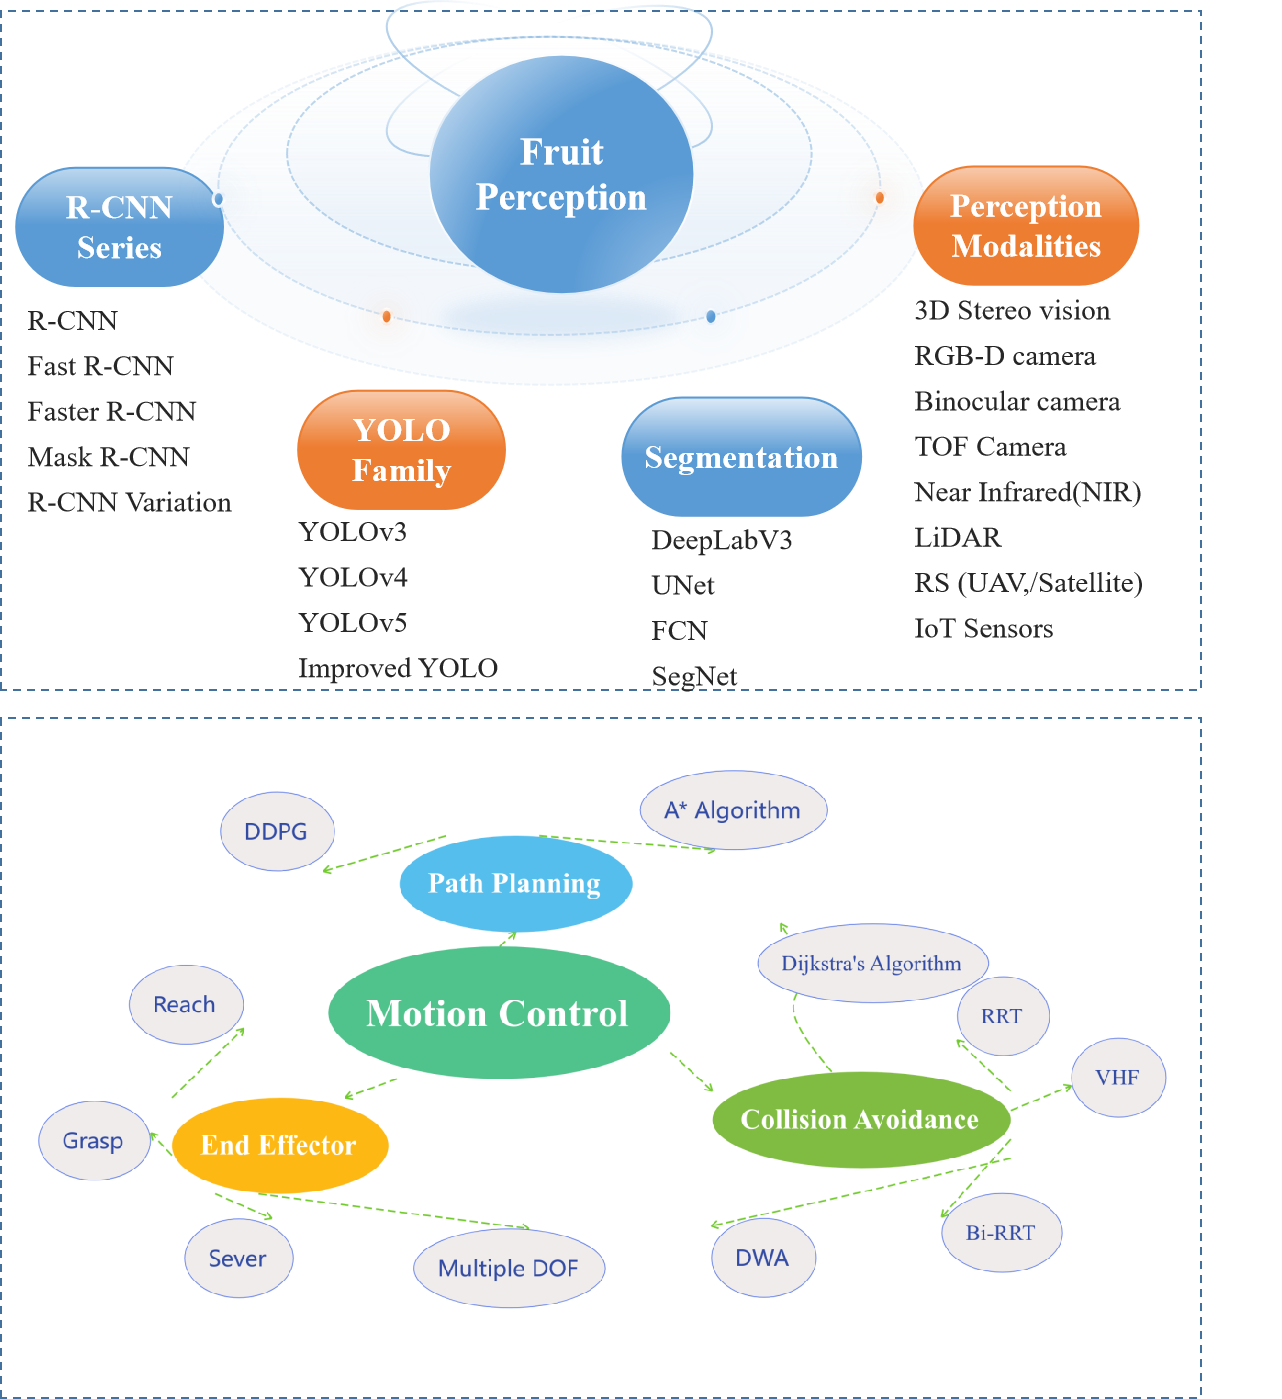
\includegraphics[width=0.55\textwidth]{fig_struct2.png}
    \caption{The perception-action framework of autonomous Fruit-Picking robots.}
    \label{fig:struct}
\end{figure}

\begin{table*}[htbp]
\centering
\footnotesize
\caption{Expanded Review Scope and Core Contributions of Major Fruit-Picking Robot Survey Papers}
\renewcommand{\arraystretch}{1.2}
\begin{tabular}{
    p{0.03\textwidth}  % Ref.
    p{0.075\textwidth}  % Year Range
    *{7}{>{\centering\arraybackslash}p{0.07\textwidth}} % Focus Scope x7
    p{0.22\textwidth}   % Summary
}
\hline
\multirow{2}{*}{\textbf{Ref.}}
& \multirow{2}{*}{\textbf{Range}}
& \multicolumn{7}{c}{\textbf{Focus Scope}}
& \multirow{2}{*}{\textbf{Trends}} \\
\cline{3-9}
&& \footnotesize Percep. Sensors
& \footnotesize Machine Vision
& \footnotesize Motion Planning
& \footnotesize End-Effectors
& \footnotesize Mechanical Automation
& \footnotesize System Integration
& \footnotesize Field Adaptation
& \\
\hline
\cite{hou2023overview}      & 2001-2022
& \ensuremath{\checkmark} & \ensuremath{\checkmark} & \ensuremath{\times} & \ensuremath{\times} & \ensuremath{\times} & \ensuremath{\times} & \ensuremath{\times}
& Deep learning fusion \\

\cite{zhang2024automatic}   & 1968-2023
& \ensuremath{\times} & \ensuremath{\checkmark} & \ensuremath{\checkmark} & \ensuremath{\checkmark} & \ensuremath{\checkmark} & \ensuremath{\checkmark} & \ensuremath{\checkmark}
& End-to-end automation \\

\cite{navas2021soft}        & 1993-2021
& \ensuremath{\times} & \ensuremath{\times} & \ensuremath{\times} & \ensuremath{\checkmark} & \ensuremath{\times} & \ensuremath{\times} & \ensuremath{\times}
& Soft gripping advances \\

\cite{zhou2022intelligent}  & 2012-2021
& \ensuremath{\times} & \ensuremath{\checkmark} & \ensuremath{\checkmark} & \ensuremath{\times} & \ensuremath{\times} & \ensuremath{\times} & \ensuremath{\checkmark}
& Modular architecture \\

\cite{mingyou2024orchard}   & 2003-2023
& \ensuremath{\times} & \ensuremath{\checkmark} & \ensuremath{\checkmark} & \ensuremath{\times} & \ensuremath{\checkmark} & \ensuremath{\checkmark} & \ensuremath{\checkmark}
& Multi-robot perception \\

\cite{rajendran2024towards} & 1995-2022
& \ensuremath{\checkmark} & \ensuremath{\checkmark} & \ensuremath{\times} & \ensuremath{\checkmark} & \ensuremath{\times} & \ensuremath{\times} & \ensuremath{\checkmark}
& Precision harvesting \\
This work & 2015-2024
& \ensuremath{\checkmark} & \ensuremath{\checkmark} & \ensuremath{\checkmark} & \ensuremath{\checkmark} & \ensuremath{\checkmark} & \ensuremath{\checkmark} & \ensuremath{\checkmark}
& Perception-action integration, \newline Multimodal integration \\
\hline
\end{tabular}
\label{tab:survey_summary}
\end{table*}

\iffalse
Existing reviews summarized in Table~\ref{tab:survey_summary} have laid valuable groundwork in autonomous fruit-picking robotics, however, they predominantly focus on fragmented components: individual sensor deployments (e.g., IoT or remote sensing in isolation \cite{mohamed2021smart,martos2021ensuring}), standalone model advancements (e.g., MTA-YOLACT for segmentation \cite{li2023mta}), or single-algorithm path planning (e.g., hierarchical trajectory methods \cite{liu2024hierarchical}). 
%While these works have advanced understanding of multi-sensor fusion, DL-based detection, and motion control techniques, 
They lack a critical systems-level perspective—failing to address how these components interact as an integrated ecosystem.
Notably, prior reviews overlook three pivotal gaps: (1) they rarely explore how multi-sensor fusion (e.g., LiDAR-vision integration \cite{liu2024hierarchical}) can be strategically paired with DL models to enhance robustness against real-world variability like occlusion or lighting changes; (2) they insufficiently connect visual perception (e.g., ripeness detection \cite{hou2023overview}) to context-aware motion planning tailored for unstructured orchards; and (3) they neglect the end-to-end optimization of collaborative systems (e.g., multi-arm coordination \cite{li2023multi}) that bridge perception, planning, and actuation.

This survey addresses these limitations by adopting a holistic "perception-action" framework. It uniquely emphasizes the synergistic integration of: (1) multi-modality sensor fusion (combining IoT, remote sensing, and vision \cite{mohamed2021smart,martos2021ensuring,liu2024hierarchical}) with DL models (e.g., evolved YOLO architectures) to mitigate detection fragility in dynamic environments; (2) visual perception outputs (e.g., fruit stem localization \cite{li2023mta}) with adaptive path planning (e.g., LiDAR-fused trajectory optimization \cite{liu2024hierarchical}) for seamless operation in unstructured terrain; and (3) collaborative robotics principles \cite{lytridis2021overview,li2023multi} with system-level efficiency analysis to address scalability challenges.


The core contributions of this survey are thus:
\begin{itemize}
\item A systematic analysis of how multi-sensor fusion strategies can be optimally aligned with DL models to enhance detection robustness across diverse agricultural scenarios, filling the gap in fragmented sensor-model discussions.
\item  A comprehensive quantitative analysis on fruit detection models, systematically comparing architectural trade-offs in accuracy (e.g., 87.83\%-99.5\% AP and efficiency (e.g., 5 ms-0.467 s per image) across diverse agricultural scenarios, and establishing decision frameworks for model selection based on specific orchard characteristics (such as greenhouse/outdoor environments, fruit density, and lighting conditions).
\item A systematic dissection of three core performance metrics (reliability, precision, rapidity) in fruit detection over the past decade, quantifying their strengths (e.g., 96\% detection rate for ripe tomatoes via color-based methods, 28 ms/image inference speed for apples) and limitations (e.g., 5.27\% relative error in occluded citrus contour analysis, speed-accuracy trade-off in small fruit detection), while establishing interconnections between metrics to guide holistic performance optimization in agricultural robotics.
\item A comprehensive synthesis of robotic motion control systems for fruit harvesting , spanning diverse fruits (apple, sweet pepper, strawberry, etc.) and control strategies (multi-DOF manipulators, dual-arm coordination, visual servoing), which quantifies performance gaps (e.g., 18-84\% success rate variance, 4-24 s cycle time range) and identifies critical interconnections between motion planning algorithms, environmental complexity, and harvesting efficiency to guide robotic system optimization in unstructured agricultural settings.
%\item An integrated exploration of perception-to-action pipelines, connecting visual insights to motion planning algorithms specifically tailored for orchard complexity.
%\item A critical evaluation of collaborative robotic systems that unify multi-arm coordination with cost-effective design principles, addressing scalability barriers overlooked in prior component-focused reviews.
\end{itemize}
\fi

The main structure of this paper is outlined in Figure \ref{fig:struct}; accordingly, the remainder of the review is organized as follows. Section II describes the overall methodology, including the search strategy, paper selection, and synthesis of findings. Section III provides a synthesis and comparative discussion of data acquisition approaches through multi-sensor fusion.
%analysis of existing fruit-picking methodologies, focusing on emerging challenges, the evolution of AI vision methods, and strategies to overcome limitations in detection and motion planning. 
Section IV discusses advances in visual perception for fruit-picking robotics, covering state-of-the-art vision models (including R-CNN, YOLO, and segmentation), and core performances metrics of fruit-picking robotics. Section V reviews advances and trends in motion control for robotic fruit harvesting, emphasizing algorithmic path planning, obstacle avoidance, and developments in motion planning and control. Section VI presents recent progress and future directions in autonomous fruit harvesting technologies. Finally, Section VII concludes the paper, summarizing key findings and outlining prospects for future research.



\section{Survey Methodology}
This survey adheres to the Preferred Reporting Items for Systematic Reviews and Meta-Analyses (PRISMA) guidelines \cite{page2021prisma} to ensure a transparent and thorough literature review.  Following PRISMA guidelines, our process began with comprehensive database searches to identify relevant literature on autonomous fruit-picking robots. 
%The primary objective is to identify and analyze highly cited papers that have significantly contributed to the field of fruit-picking robotics, the outline of which is shown in Figure~\ref{fig:prisma1}.
% The methodology consists of several stages: defining search criteria, selecting relevant papers, extracting data, and synthesizing the findings.
%To enhance the clarity, coherence, and conciseness of the survey, the AI language model ChatGPT, developed by OpenAI, was employed. 
%To improve clarity, coherence, and conciseness, we employed the AI language model ChatGPT (developed by OpenAI) for rephrasing and summarizing. ChatGPT assisted in rephrasing text, ensuring each paragraph flowed seamlessly into the next and the overall narrative maintained a professional tone. The model was also used to generate summaries of individual papers, which were then reviewed and refined to match the context and requirements of this survey. The integration of ChatGPT into the writing process helped streamline the content organization and improve the paper's readability. The utilization of ChatGPT in academic writing has been discussed in detail by Gruda and Dritjon~\cite{gruda2024three}.
\begin{figure}[h!]
    \centering
    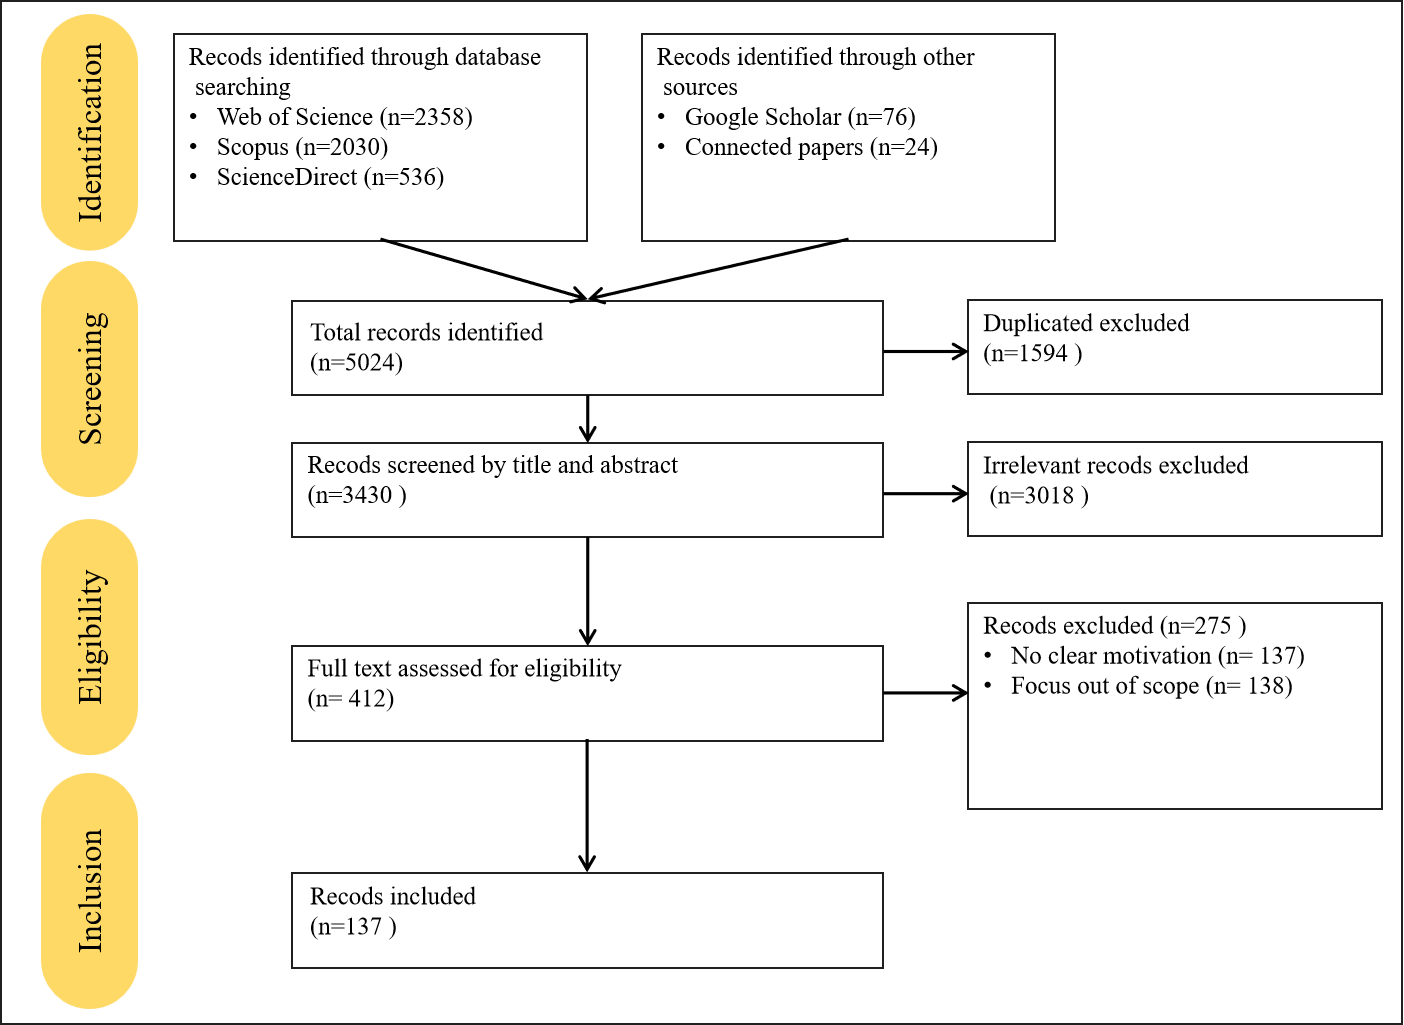
\includegraphics[width=0.5\textwidth]{fig_prisma1.png}
    \caption{ PRISMA flowchart illustrating the literature selection process for the survey on autonomous fruit-picking robots. 
    %Flow diagram depicting the identification and selection of publications to be included in this review.
    }
    \label{fig:prisma1}
\end{figure}

%Following PRISMA guidelines, our process began with database searches
We searched major academic databases, including Scopus, Web of Science (WoS) and ScienceDirect, using targeted keywords and phrases related to fruit-picking robotics. Table~\ref{tab:keywords} lists the search strings employed, which combined terms such as "autonomous fruit picking," "robotic harvesting," "deep learning in orchard," to capture a broad range of studies from 2015 to 2024. This initial search yielded 3,430 records after removing duplicates.
%We began our research by systematically searching three well-established scientific databases, Web of Science (WoS), ScienceDirect and Scopus, to assemble a comprehensive collection of publications related to autonomous fruit-picking robots. The keywords used for these searches are listed in Table~\ref{tab:keywords}. The search was limited to English-language articles published between 2015 and 2024. This process resulted in 2358 records from WoS, 536 from ScienceDirect and 2030 from Scopus, as well in 100 from Google Scholar and Connected Papers, for a combined total of 4924 records prior to screening. To further ensure the completeness of our dataset, we also performed supplementary searches via Google Scholar and the Connected Papers , yielding an additional 76 and 24 records, respectively. In total, 5024 publications were identified in this initial phase.

%Of the 5024 records initially identified, a comprehensive screening process was conducted to ensure the quality and relevance of the included studies. First, duplicates were identified and removed, resulting in 3430 unique entries. Manual screening was then performed without the aid of automation tools. During the title screening phase, 3018 records were excluded based on apparent irrelevance to the review topic. The remaining studies underwent abstract screening, which further reduced the collection to 412 potentially relevant records. Finally, full-text reviews were conducted on these entries to assess their fit with the review criteria.

\begin{table}[ht]
\scriptsize
\caption{Keywords and Criteria Used in Preliminary Database Search.} 
\label{tab:keywords} 
\begin{tabular}{p{0.3\linewidth} p{0.5\linewidth}}
\hline
\textbf{Criteria} & \textbf{Terms} \\ \hline
\textbf{Database}  &  Web of Science, Scopus, ScienceDirect \\
\textbf{Search Field} & Title, Keywords and Abstract\\
 & fruit-picking robot or autonomous fruit-picking robot  or robotics harvesting or harvesting robot or deep learning in orchard\\
\textbf{Language} & English \\
\textbf{Publication Date} & From 2015 TO 2024 \\ \hline 
\end{tabular}
\end{table}

Subsequent screening applied predefined inclusion and exclusion criteria to refine the selection. Inclusion criteria encompassed:

(1)Records describing advancements in perception, motion control, or end-to-end systems for fruit-picking robots;

(2)Studies published in peer-reviewed journals or conferences between 2015 and 2024;

(3)Works providing empirical evaluations or novel methodologies in agricultural robotics.

Exclusion criteria included:

(1)Non-English publications;

(2)Records focused solely on non-fruit crops or unrelated agricultural tasks;

(3)Grey literature without rigorous peer review.

After title and abstract screening, 412 records advanced to full-text review, resulting in 152 studies selected for in-depth analysis. Figure \ref{fig:prisma1} presents the PRISMA flowchart, detailing the number of records at each stage of the screening process, from initial identification to final inclusion.

To improve clarity, coherence, and conciseness in the presentation of findings, we employed the AI language model ChatGPT as a tool for rephrasing and summarizing complex sections \cite{gruda2024three}. This assistance was integrated post-analysis to refine the manuscript without altering the underlying data or interpretations, ensuring the content remained grounded in the reviewed literature.

%The inclusion criteria for this review were as follows: (i) records describing fruit picking methods involving visual detection and segmentation; (ii) records focused on robot motion control applications such as path planning and collision avoidance; (iii) explicit statements regarding the motivation behind agricultural robot harvest; (iv) Records focused on the development, application, and evaluation of harvesting robots; (v) publications in the form of journal articles or conference proceedings; and (vi) empirical research based on experimental results rather than purely simulation-based studies.

%Papers were excluded if they: (i) did not meet the above inclusion criteria; (ii) were review articles, surveys, or book chapters; (iii) lacked a clearly articulated motivation for agriculture robot; (iv) relied solely on simulation without experimental validation; or (v) were unavailable or inaccessible in full text.

%\section{Data Acquisition Through Multi-Sensor Fusion}
\section{Multi-Sensor Fusion and Modality Synergy in Robotic Fruit Picking}
%Modern fruit-picking robotics increasingly relies on a diverse array of sensor technologies such as 3D stereo vision, RGB-D cameras, binocular vision, as well as integration with IoT, GIS, laser, and RS to obtain robust environmental and positional data. As summarized in 
%Figure~\ref{fig:camera}, these combined methodologies enable more exhaustive and accurate perception, greatly enhancing fruit detection and localization even in challenging agricultural conditions.

Modern fruit-picking operations are increasingly reliant on precise measurements of plant morphology and depth. Plant morphology encompasses features such as color, shape, edge, 	3D contour, texture, and ripeness of fruits, leaves, peduncle and stems under varying illumination, occlusion, and dynamic conditions—characteristics primarily captured by various visual sensors. For depth characterization of observed targets, distance sensors are additionally required. 
Consequently, fruit-picking robots rely on multi-sensor fusion (as illustrated in Figure ~\ref{fig:camera}) to acquire diverse features, thereby reducing measurement errors and enhancing robustness.
%Consequently, fruit-picking robots inevitably depend on multi-sensor fusion to acquire these diverse features, as illustrated in Figure~\ref{fig:camera}. Furthermore, the synergy among different modalities effectively reduces measurement range errors, enhances robustness, adaptability, and precision under illumination variations and occlusion, shortens picking time, and improves real-time performance.
\begin{figure}[hbtp]
\centering
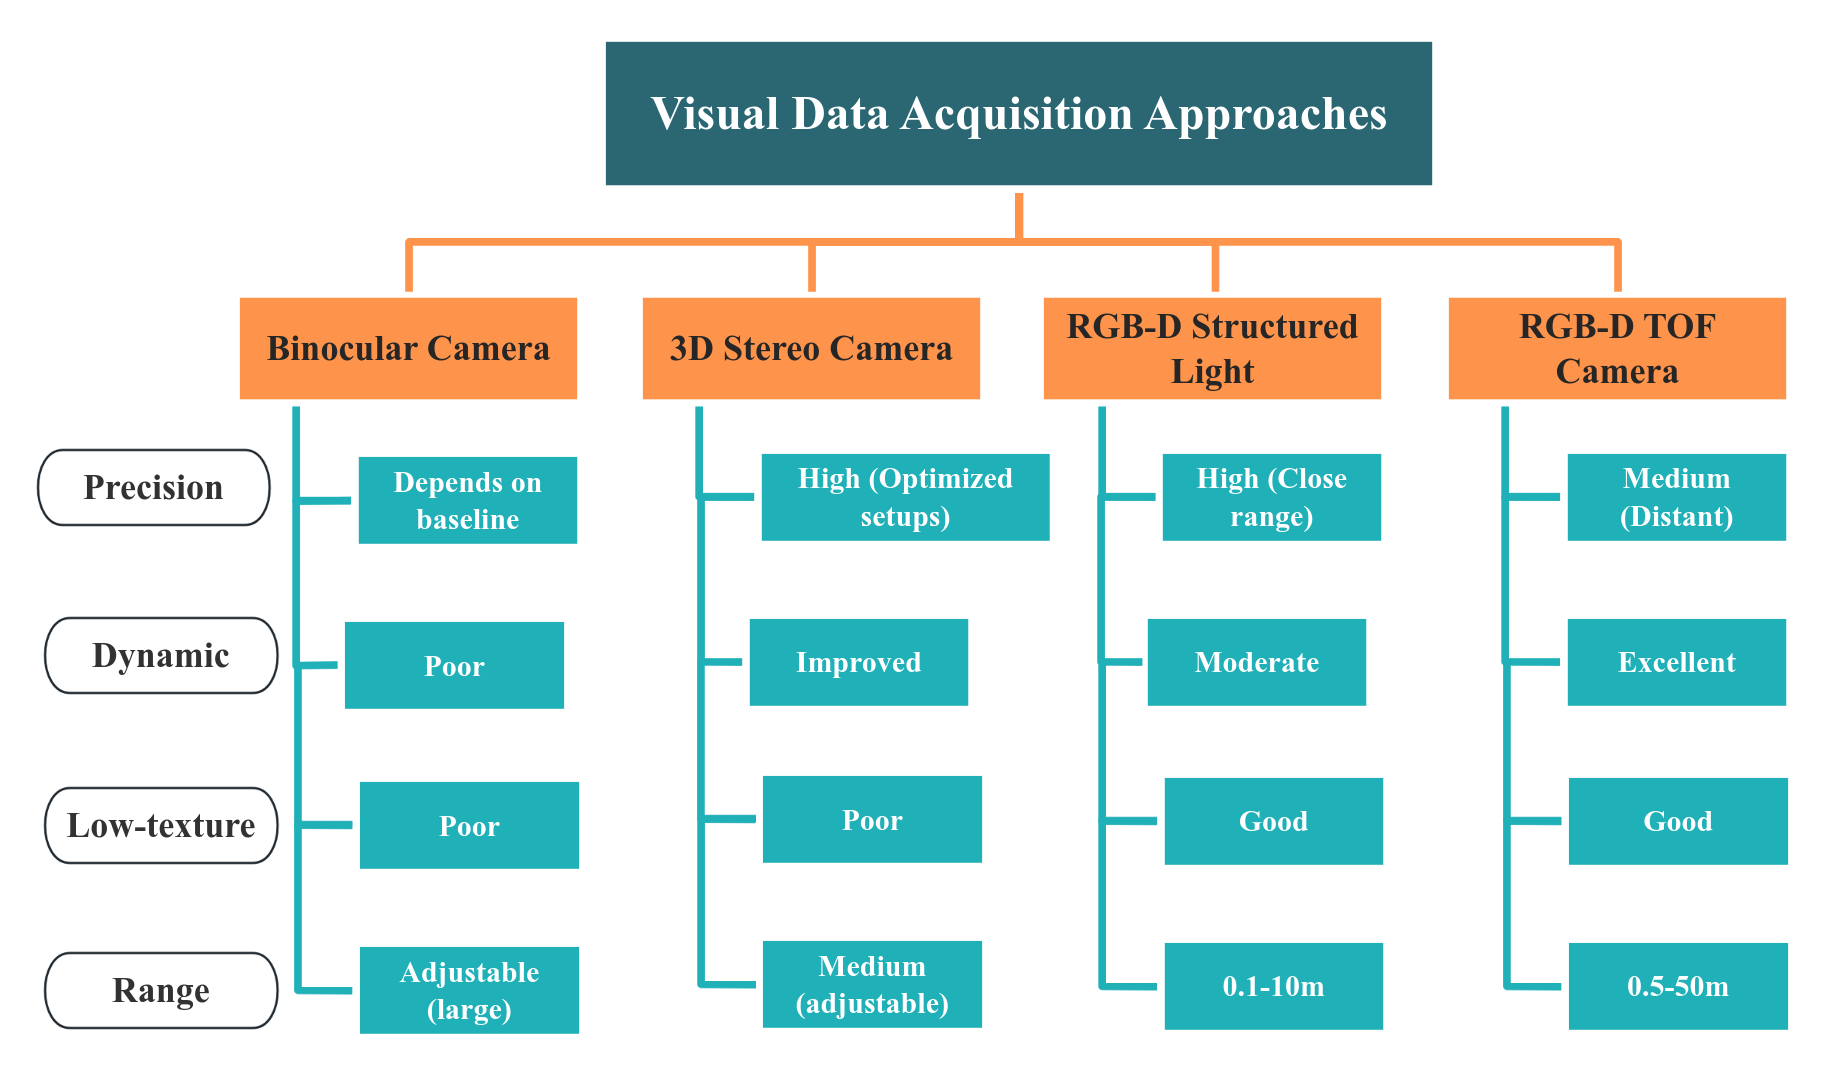
\includegraphics[width=0.52\textwidth]{fig_camera1.png}
\caption{Overview and comparison of four mainstream visual data acquisition methods, highlighting their key performance characteristics for object detection.}
\label{fig:camera}
\end{figure}

\begin{table*}[ht]
\scriptsize
\centering
\caption{Multi-Sensor Fusion and Multi-Modality Synergy in Orchard Applications} 
\label{tab:dataset}
%\begin{tabular}{p{0.02\textwidth}p{0.02\textwidth}p{0.10\textwidth}p{0.04\textwidth}p{0.07\textwidth}p{0.16\textwidth}p{0.18\textwidth}p{0.12\textwidth}p{0.10\textwidth}}
\begin{tabular}{p{0.02\textwidth}p{0.02\textwidth}p{0.13\textwidth}p{0.04\textwidth}p{0.07\textwidth}p{0.16\textwidth}p{0.23\textwidth}p{0.14\textwidth}}
\hline
%\textbf{Ref.} & \textbf{Year} & \textbf{Sensor Fusion} & \textbf{Fruit} & \textbf{Orchard} & \textbf{Multi-Modality Synergy} & \textbf{Key Advantages} & \textbf{Limitations} & \textbf{Application} \\ 
\textbf{Ref.} & \textbf{Year} & \textbf{Sensor Fusion} & \textbf{Fruit} & \textbf{Orchard} & \textbf{Multi-Modality Synergy} & \textbf{Strengths} & \textbf{Limitations} \\ 
\hline
\cite{wang2016localisation} & 2016 & Binocular CCD + Laser rangefinder & Litchi & Unstructured & Visual features (RGB) + spatial calibration (laser) & High adaptability to illumination variations and occlusion (94\% matching rate for partial occlusion) & Processing time (3213 ms) \\ 
\hline
\cite{si2015location} & 2015 & Binocular CMOS + Laser rangefinder & Apple & Unstructured & Color segmentation (RGB) + depth calibration (laser) & Robust under varying light (97.9\% cloudy, 89.5\% backlight) & Limited to 400–1500 mm range  \\ 
\hline
\cite{luo2016vision} & 2016 & Binocular CMOS + Calibration board & Grape & Vineyard & Stereo matching (RGB) + parameter calibration & Real-time performance (<0.7 s) with 87\% detection rate & Limited to 350–1100 mm range  \\ 
\hline
\cite{barnea2016colour} & 2016 & RGB camera + SwissRanger4000 & Pepper & Greenhouse & Highlight pruning (RGB) + 3D symmetry (depth) & Color-agnostic detection (mean average precision (mAP) 0.55), robust to occlusions & Slow processing (197 s per image)  \\ 
\hline
\cite{gongal2018apple} & 2018 & CCD camera + TOF camera + Laser & Apple & Commercial & RGB segmentation + 3D spatial analysis + pixel size modeling & High accuracy in size estimation (84.8\%) & Requires controlled lighting (tunnel + LED) \\ 
\hline
\cite{gene2019fruit} & 2019 & LiDAR (Velodyne VLP-16) + RTK-GNSS & Apple & Commercial & Reflectance analysis (LiDAR) + absolute positioning (GNSS) & Sunlight-insensitive with 87.5\% localization success & High equipment cost  \\ 
\hline
\cite{kusumam20173d} & 2018 & Kinect 2 + LED lighting & Broccoli & Outdoor & 3D geometry (depth) + color stability (LED) & High precision (95.2\%) across weather conditions & Low depth resolution (512×424)  \\ 
\hline
\cite{andujar2016using} & 2016 & Kinect v1 + Skanect3D software & Cauli- flower & Commercial & RGB segmentation + 3D volume modeling & Non-destructive yield estimation ($R^2$=0.87) & Limited to 640×480 resolution \\ 
\hline
\cite{onishi2019automated} & 2019 & ZED stereo camera + UR3 robotic arm & Apple & V-shaped & SSD detection (RGB) + 3D triangulation + robotic control & High detection rate (92.31\%) with 16 s/fruit harvesting & Only for partial occlusion \\ 
\hline
\cite{underwood2016mapping} & 2016 & LiDAR (SICK LMS-291) + RGB camera + GPS & Almond & Commercial & 3D canopy modeling (LiDAR) + flower/fruit density (RGB) & Efficient orchard mapping (6.2 km in 1.5 h) & Limited to large-scale orchards  \\ 
\hline
\cite{koenig2015comparative} & 2015 & LiDAR (Riegl VZ-400) + Hyperspectral system & Barley & Post-harvest & Geometric features (LiDAR) + radiometric calibration (hyperspectral) & High classification precision (99\%) for post-harvest growth & Requires Spectralon calibration target  \\ 
\hline
%\cite{li2023multi} & 2023 & 4×Intel RealSense D435i RGBD cameras & Apple & SNAP orchard (dwarf dense) & RGB+depth via multi-task DCNN; frustum-based point cloud processing; global fruit map fusion & Reduced median position error by 44.43\%; 71.28-80.45\% harvest success; 5.8-6.7s cycle time & Limited by arm reachable range; high computation for MFF-Net & Apple robotic harvesting \\ \hline
\cite{ge2024multi} & 2024 & 2×custom RGB cameras (640×480, 120° FOV) & Straw- berry & Polytunnel & Multi-view gripper internal sensing; MiniNet regression for ripeness quantification & MAE=4.8\% (Huber loss); 6.5ms inference time; full-view coverage & Annotation subjectivity; coefficient determination for fusion needs improvement \\
\hline
\cite{chen2024mlp} & 2024 & Azure Kinect (RGB+depth+ NIR) & Tomato & Greenhouse & MLP-based fusion encoder (RGB+depth+NIR); YOLO-DNA framework & mAP@0.5=98.13\%; 37.12 FPS; robust to illumination variations & MLP computation slower on GPU; needs more data for generalization  \\
\hline
%\cite{sadeghian2025reliability} & 2025 & LiDAR+6×cameras & - & Autonomous driving (fruit-picking extension) & BEV space fusion; STFA for temporal consistency; CW-MCA with reliability scores & mAP=70.6\%; robust to sensor malfunctions (LiDAR FOV limitation/50\% drop) & Designed for driving, needs adaptation to orchard dynamics & 3D object detection for mobile picking robots \\ \hline
\end{tabular}
\end{table*}

Among multi-sensor approaches, 3D stereo vision systems are essential by using dual cameras to estimate depth via triangulation, effectively mimicking human binocular vision. Early efforts include Wang et al.~\cite{wang2016localisation}, who developed a binocular stereo vision system for litchi localization, incorporating wavelet transforms and clustering methods to achieve high accuracy under natural lighting. Similarly, Si et al.~\cite{si2015location} advanced apple detection by enabling their stereo vision platform to recognize and localize multiple fruits simultaneously in variable environments. Luo et al.~\cite{luo2016vision} further demonstrated a grape-harvesting stereo system capable of quickly detecting cutting points and estimating yields with high efficiency.
RGB-D cameras which combine color information with depth sensing using time-of-flight or structured light have also proven highly beneficial. Barnea et al.~\cite{barnea2016colour} presented an RGB-D-based 3D detection method capable of analyzing both shape and symmetry, which is effective for sweet pepper harvesting even under complex conditions. Nguyen et al.~\cite{nguyen2016detection} showed that integrating depth with RGB data significantly improves apple detection and localization, especially under occlusion. Kusumam et al.~\cite{kusumam20173d} and Andújar et al.~\cite{andujar2016using} extended these principles to broccoli and cauliflower, using mobile RGB-D platforms to deliver precise 3D crop measurements crucial for automated harvest scheduling.
Sensor fusion extends beyond vision alone: for example, Gongal et al.~\cite{gongal2018apple} used a combination of color and time-of-flight 3D cameras to estimate apple size, demonstrating higher accuracy using pixel size information—an important step forward for volume estimation and crop management.
The integration of visual sensors with advanced algorithms—such as DL models and inverse kinematics—further automates and optimizes fruit detection and harvesting. Onishi et al.~\cite{onishi2019automated} combined a stereo camera with an SSD DL model to achieve high real-time detection accuracy, precisely guiding the robot’s arm through calculated movements.

%Multi-modality data fusion plays a critical role in advancing agricultural robotics by enhancing perception accuracy and operational efficiency. 
While multi-sensor systems, such as 3D stereo vision setups, have significantly advanced agricultural robotics by capturing richer environmental data, their effectiveness remains constrained when relying solely on homogeneous sensor inputs (e.g., visual data from dual cameras). To address this limitation, multi-modality data fusion has emerged as a logical next step, extending beyond the integration of similar sensors to combine fundamentally different types of data. This approach leverages the unique strengths of diverse modalities including visual, spectral, IoT-derived etc. to create a more comprehensive and robust perceptual framework.
For example, Horng et al.~\cite{horng2019smart} developed a crop harvesting system that integrates image recognition with IoT technology. By combining MobileNetV2 and SSD, the system can assess crop maturity with an average precision of 84\% and coordinate the movement of multiaxial robotic arms. This integrated solution automates and optimizes harvesting procedures, leading to increased efficiency and a reduction in labor-intensive tasks.
LiDAR-based data fusion has also shown considerable promise in orchard-scale mapping and monitoring. Underwood et al.~\cite{underwood2016mapping} demonstrated the integration of LiDAR and vision sensors on a mobile robotic platform for almond orchard mapping. This approach enables dynamic 3D mapping of canopy volumes, as well as the capture of data on flower and fruit densities, facilitating automated and season-spanning monitoring. The system revealed a strong predictive correlation between sensor-derived canopy volumes and actual yields, establishing a benchmark for subsequent developments in field robotics.
Further highlighting the advantages of LiDAR technology, Gené-Mola et al.~\cite{gene2019fruit} utilized a mobile terrestrial laser scanner equipped with a Velodyne VLP-16 to detect and localize Fuji apples by analyzing reflectance at 905 nm. The method achieved a localization success rate of 87.5\%, an identification success rate of 82.4\%, and an F1-score of 0.858, demonstrating robust performance under various lighting conditions and precise three-dimensional fruit localization. Koenig et al.~\cite{koenig2015comparative} conducted a comparative analysis of post-harvest growth detection using terrestrial LiDAR point clouds, achieving 99\% precision with 0.0\% error. Their work underscores the effectiveness of combining geometric and radiometric features and demonstrates the utility of LiDAR in weed management for precision agriculture.

Collectively, as illustrated in Table~\ref{tab:dataset}, multi-modality synergy enhances the capabilities of fruit-picking robots by providing accurate data for detection and harvesting, though limitations persist in diverse agricultural applications
%Collectively, as illustrated in Table~\ref{tab:dataset}, multi-modality synergy enhance the capabilities of fruit-picking robots by providing the necessary data for accurate fruit detection, efficient harvesting, and robust operation besides existed limitations for diverse application in agricultural environments .

\section{Advances in Visual Perception for Fruit-Picking Robotics}
%We explores the latest advancements in fruit-picking robotics, focusing on three key areas: popular technologies in fruit detection and classification, and challenges-oriented solutions and applications. In the following section, an examination is conducted of the prominent technologies utilised in the detection of fruit, including segmentation models, the R-CNN series, and the YOLO series, in addition to other innovative classification approaches. Finally, we address the practical challenges in deploying fruit-picking robots, such as accurate pick-point detection, ripeness recognition, and efficiency in diverse conditions, and review the solutions proposed to overcome these obstacles. Collectively, these advancements underscore the substantial progress achieved in the field and its considerable potential for transforming agricultural practices.
Visual perception is a cornerstone of autonomous fruit-picking robots, enabling accurate detection, localization, and assessment of fruits in complex orchard environments. 
Building upon established methodologies for multi-sensor and multi-modal data acquisition, particular emphasis is placed on the critical processes of data identification and segmentation. 
Leading techniques include the R-CNN family and YOLO series, which excel in object detection and segmentation.
In addition, segmentation-specific models contribute to the refined delineation of target entities, enabling more precise extraction of relevant information. An extensive review of the current literature reveals the application of these models in areas such as pinpointing harvesting locations, assessing fruit ripeness, optimizing operational efficiency, and recognizing parameters including object color, shape, and contour.
By building narrative connections between these methodologies, we highlight their evolutionary synergies and applications in robotic harvesting.
 % By synthesizing insights from diverse research developments, this analysis delineates recent advancements and identifies prospective directions for innovation in agricultural data processing.


\subsection{R-CNN Family: Foundations of Instance Segmentation}
The R-CNN family has been pivotal in establishing robust instance segmentation for fruit detection, where individual fruits are identified and delineated from cluttered backgrounds. Early iterations, such as Fast R-CNN, improved efficiency by sharing convolutional features across region proposals, achieving higher accuracy in distinguishing fruits from leaves or branches under varying lighting conditions.
%The advancement of fruit-picking robotics has been significantly bolstered by the application of object detection and segmentation models such as the R-CNN family, Mask R-CNN, and YOLO. Each of these technologies addresses the challenges of complex agricultural environments, enhancing both the accuracy and efficiency of fruit localization, identification, and harvesting decisions. Over time, these models have evolved to balance detection precision with real-time computational demands, making them increasingly suitable for automated agricultural applications.
\begin{figure}[hbtp]
\centering
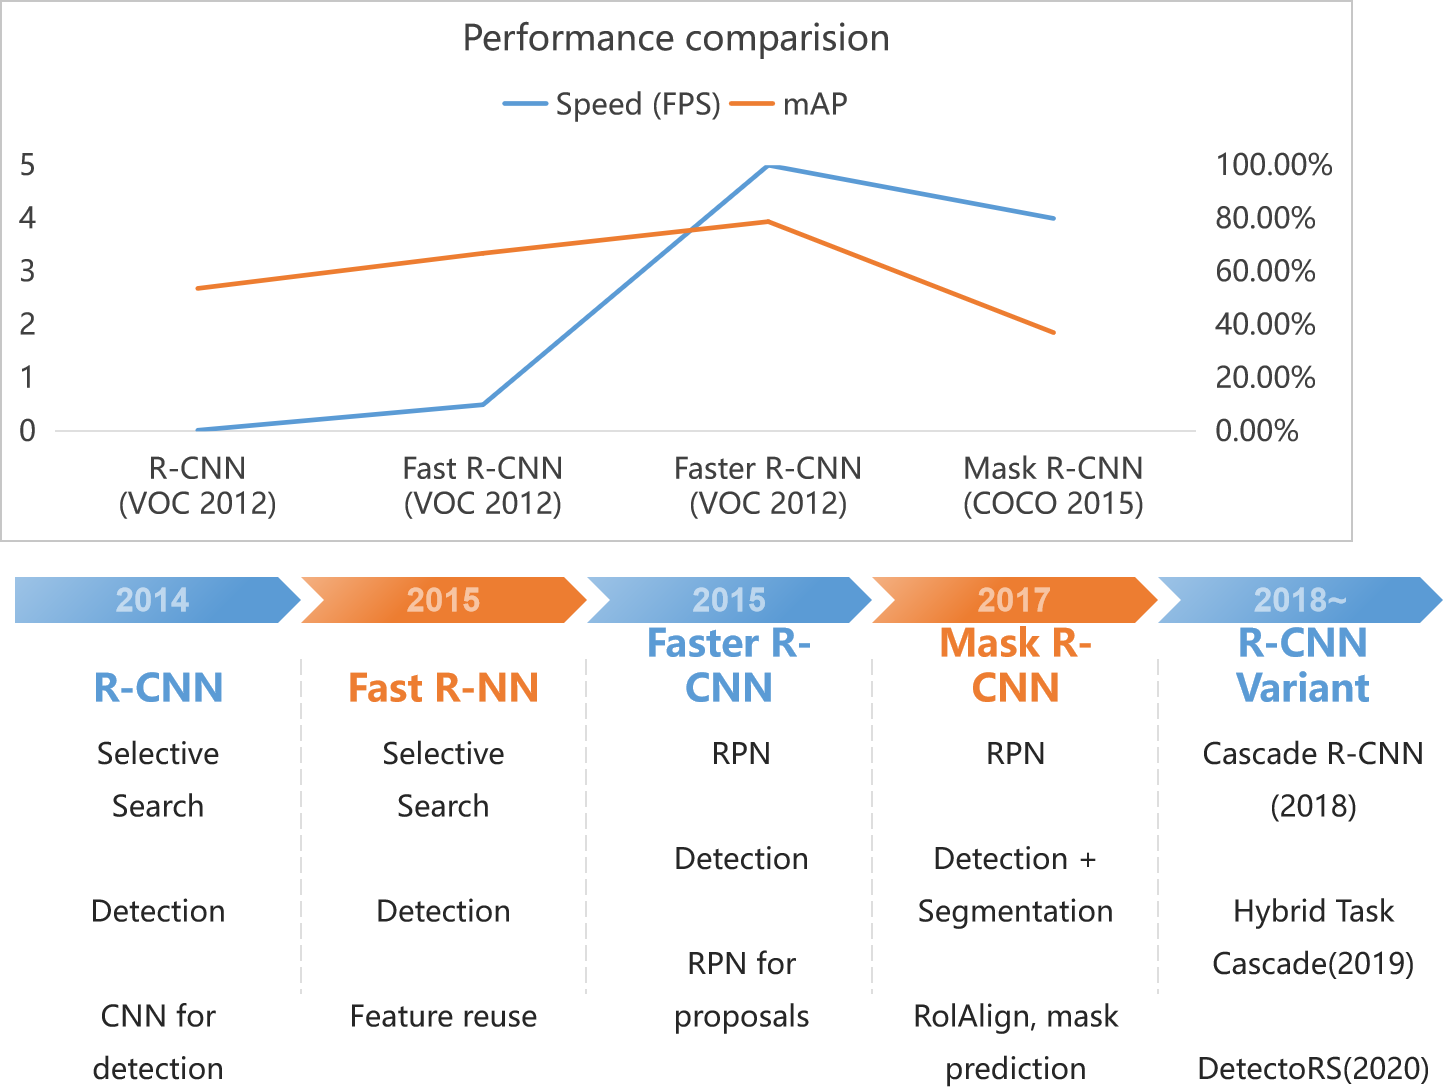
\includegraphics[width=0.5\textwidth]{fig_rcnn1.png}
\caption{The performance of R-CNN family for object detection.}
\label{fig:performance_rcnn}
\end{figure}

%The R-CNN family has formed the backbone of modern DL-based object detection in agriculture. 
The original R-CNN, introduced in 2014~\cite{girshick2014rcnn}, pioneered the use of selective search to generate region proposals, followed by CNN-based feature extraction and SVM classification. Despite its improved detection accuracy, R-CNN's computational inefficiency—due to processing thousands of proposals per image—limited its real-time applicability.
To addressed these bottlenecks by sharing the convolutional computation across the entire image and using Region of Interest (RoI) pooling, Girshick~\cite{girshick2015fast} introduced Fast R-CNN in 2015, significantly expediting both training and inference. By sharing features across region proposals, it achieved a remarkable speed-up (e.g., ~2.3s/image compared to R-CNN's 47s/image) and higher accuracy (mAP=66.9\% on PASCAL VOC). However, it still relied on the time-consuming selective search for region proposal generation.
Subsequently, Ren et al. ~\cite{ren2015faster} presented Faster R-CNN in 2015, further integrated the detection pipeline by introducing a Region Proposal Network (RPN) directly within the convolutional architecture, which replaced selective search and enabled full end-to-end training. Faster R-CNN achieved a speed of ~0.2s/image and a mAP of ~78.8\% on PASCAL VOC, balancing speed and accuracy well. Despite its success, the RoI Pooling in Faster R-CNN introduced quantization errors. 
%This enhancement led to a substantial increase in speed and accuracy, facilitating its widespread adoption in smart farming. 
Later, Sa et al.~\cite{sa2016deepfruits} applied Faster R-CNN for multi-modal fruit detection, demonstrating its adaptability by fusing RGB and near-infrared data, resulting in robust performance under variable field conditions and reducing the annotation workload. Similarly, Wan et al.~\cite{wan2020faster} optimized Faster R-CNN with a self-learning image library and advanced data augmentation to improve detection speed and accuracy across multiple fruit types, achieving a mAP exceeding 91\%.
Recent research has extended Faster R-CNN to incorporate additional modalities and tailored architectures. Fu et al.\cite{fu2020faster} augmented the framework using RGB-D imaging for apple detection in dense orchards, while Tu et al.~\cite{tu2020passion} proposed a multi-scale Faster R-CNN variant (MS-FRCNN) for small passion fruit recognition, combining color and depth data to handle occlusions and illumination changes. Additional studies have demonstrated the efficacy of these advanced models for kiwifruit detection~\cite{fu2018kiwifruit}, improved detection in occluded and mixed scenarios~\cite{gene2019multi, mu2020intact}, and integration with radiometric data for enhanced performance in challenging environments.

\begin{figure}[hbtp]
\centering
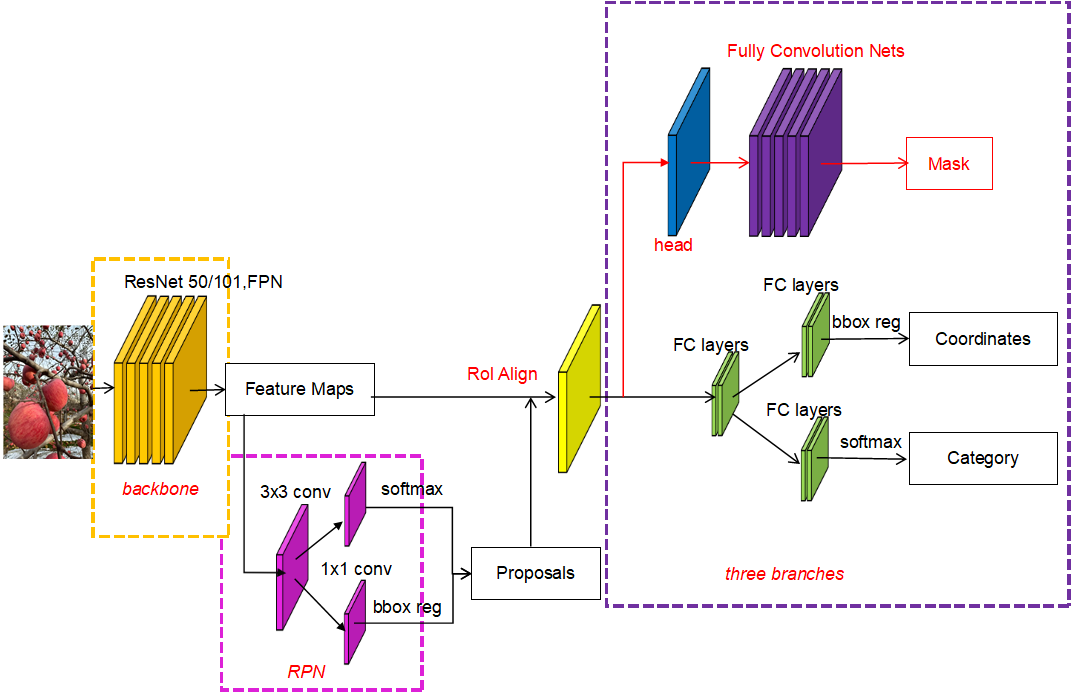
\includegraphics[width=0.5\textwidth]{fig_maskRcnn.png}
\caption{The Mask R-CNN framework for apples detection.~\cite{he2017mask}}
\label{fig:mask_rcnn}
\end{figure}

\begin{table*}[htbp]
	\centering
	\footnotesize 
	\caption{Summary of R-CNN Family Approaches for Fruit-Picking in 2015-2024 (part 1)} 
	\label{tab:RCNN-based} 
	\begin{tabular}{@{}p{0.025\textwidth}p{0.094\textwidth}p{0.084\textwidth}p{0.15\textwidth}p{0.25\textwidth}p{0.26\textwidth}@{}}
	\toprule
	\textbf{Ref. \newline /Year} & \textbf{Fruit \newline /Orchard} & \textbf{Model} & 			\textbf{Key Focus} & \textbf{Strengths} & \textbf{Limitations} \\ \midrule
	\cite{sa2016deepfruits} \newline 2016 & Multi-class (sweet pepper, rock melon, apple, etc.) \newline Outdoor/glasshouse orchards & DeepFruits (Faster R-CNN with VGG-16) & Multi-modal (RGB+NIR) fusion for cross-fruit detection & - Fusion F1: 0.838 (sweet pepper) \newline - Apple F1: 0.938; strawberry F1: 0.948 \newline - Processing time: 341–393 ms/image \newline - Requires 10–100 training images per fruit & - Early fusion underperforms (F1=0.799) vs. late fusion \newline - NIR modality alone has lower F1 (0.797) than RGB (0.816) \newline - Missed detections for small fruits (scaled <50\% of training size) \\ \midrule
	
	\cite{wan2020faster} \newline 2020 & Multi-class (apple, mango, orange) \newline Outdoor orchard & Improved Faster R-CNN (VGG-16) & Multi-class detection with optimized convolutional and pooling layers & - mAP=90.72\% across three classes \newline - Apple AP: 92.51\%, Orange AP: 90.73\% \newline - Processing speed: 58 ms/image \newline - Outperforms Faster R-CNN by 8.16\% in mAP & - Slower speed (40 ms/image) \newline - Trained on 100×100 pixel images (smaller than real-world orchard images) \newline - Limited to three fruit classes \\ \midrule

	\cite{fu2020faster} \newline 2020 & Apples (Scifresh) \newline Outdoor non-structural orchard  & Faster R-CNN (ZFNet, VGG16) & Detection using RGB and depth features with background filtering & - Foreground-RGB + VGG16: AP=0.893, processing time=0.181 s/image \newline - Depth filtering improves AP by 2.5\% (VGG16) and 2.3\% (ZFNet) \newline - VGG16 outperforms ZFNet by 10.7\% AP on Original-RGB & - ZFNet (0.124 s/image) 1.46x faster than VGG16 \newline - Kinect V2 sensitive to direct sunlight, data collected avoiding noon \newline - Foreground-RGB loses edge information due to FoV mismatch \\ \midrule
	
	\cite{tu2020passion} \newline 2020 & Passion fruits \newline Outdoor orchard & Multiple Scale Faster R-CNN (MS-FRCNN) & Detection of small passion fruits under variable lighting and occlusion & - Recall: from 0.922 to 0.962 \newline - Precision: from 0.850 to 0.931 \newline - F1-score: from 0.885 to 0.946 \newline - F1-score for small fruits: 0.909 & - No mention of processing speed \newline - Requires RGB-D camera, limiting deployment flexibility \newline - Performance might be affected by complex background beyond occlusion \\ \midrule
	
	\cite{fu2018kiwifruit} \newline 2018 & Kiwifruits \newline Outdoor non-structural orchard & Faster R-CNN (ZFNet) & Detection of clustered/occluded kiwifruits & - Overall recognition rate: 92.3\% \newline - Separated fruit recognition: 96.7\%; occluded: 82.5\% \newline - Processing time: 0.274 s/image; 5.0 ms/fruit & - Lower accuracy for occluded vs. separated fruits (14.2\% gap) \newline - Relies on bottom-view imaging to reduce overlap \newline - Training requires 40,000 iterations (about 10 hours) \\ \midrule

	\cite{gene2019multi} \newline 2019 & Fuji apples \newline Outdoor orchard (Spain) & Multi-modal Faster R-CNN (VGG-16) & Fusion of RGB, depth (D), and range-corrected intensity (S) for detection & - F1-score: 0.898; AP: 94.8\% (RGB+S+D) \newline - 4.46\% F1 improvement over RGB-only \newline - Optimal anchor scale 4 (1:1) yields 94.8\% AP \newline - Processing speed: 13.6 frames/s & - Depth sensor performance degrades under direct sunlight \newline - Single-modal depth (D) achieves low F1 (0.635) \newline - Relies on artificial lighting for data acquisition \newline - Limited to spherical small objects (44±6 px diameter) \\ \midrule
	
	\cite{mu2020intact} \newline 2020 & Immature tomatoes \newline Greenhouse & Faster R-CNN \newline (ResNet-101) & Detection of highly occluded immature tomatoes; counting, localization, and size estimation & - AP (IoU>=0.5): 87.83\% on test dataset \newline - Counting accuracy: \(R^2=0.87\) vs manual labeling \newline - Processing time: 0.37 s/image \newline - Successfully detected 1422 tomatoes in a full row & - Overfitting after 10 epochs (validation AP drops) \newline - False positives: 28.99\% of boxes <2000 pixels \newline - Underestimation when count >20 tomatoes/subimage \newline - Cannot detect fully occluded fruits (entirely shaded) \\ \midrule	
	\cite{yu2019fruit} \newline 2019 & Strawberry \newline Outdoor non-structural environment (earth-ridge cultivation)  & Mask R-CNN (ResNet50 + FPN) & Instance segmentation, picking point localization in non-structural environments (overlap, occlusion, varying illumination) & - Detection AP (95.78\%) and recall (95.41\%)\newline- MIoU for segmentation: 89.85\%\newline- Picking point localization error: ±1.2 mm (meets ±7 mm tolerance)\newline- Robust to overlap, occlusion, and illumination changes & - Processing speed (8 FPS)\newline- Unripe fruit precision (93.14\%) lower than ripe (98.41\%)  \newline- Maximum picking point error: 4 mm (malformed fruits) \newline- Relies on vertical growth assumption \\ \midrule
	\cite{jia2020detection} \newline 2020 & Apples \newline outdoor non-structural orchard & Optimized Mask R-CNN \newline (ResNet + DenseNet) & Segmentation of overlapped/occluded apples; improving real-time performance for harvesting robots & - Overall precision: 97.31\%, recall: 95.70\% \newline - Occluded fruits (>20\% area): precision 94.59\%, recall 89.74\% \newline - Outperforms existing methods in overlapping fruit detection (86.89\% vs. 85.25\% in literature) & - Relies on manual labeling (1020 images) \newline - Lower recall for heavily occluded fruits (89.74\% vs. 97.68\% for less occluded) \newline -The processing speed is not explicitly mentioned \\ 
		\bottomrule
	\end{tabular}
\end{table*}

\begin{table*}[htbp]
	\centering
	\footnotesize 
	\addtocounter{table}{-1}
	\caption{Summary of R-CNN Family Approaches for Fruit-Picking in 2015-2024 (part 2)} 
	\begin{tabular}{@{}p{0.025\textwidth}p{0.094\textwidth}p{0.084\textwidth}p{0.15\textwidth}p{0.25\textwidth}p{0.26\textwidth}@{}}
	\toprule
	\textbf{Ref. \newline /Year} & \textbf{Fruit \newline /Orchard} & \textbf{Model} & 			\textbf{Key Focus} & \textbf{Strengths} & \textbf{Limitations} \\ \midrule

	\cite{chu2021deep} \newline 2021 & Apples (Gala, Blondee) \newline Outdoor non-structural orchard & Suppression Mask R-CNN (ResNet-101-FPN) & Robust detection under varying lighting and occlusion for robotic harvesting & - F1-score: 0.905 (C1 configuration) \newline - Precision: 0.880, Recall: 0.931 (C1) \newline - Detection time: 0.25 s/frame \newline - Outperforms Mask R-CNN (ResNet152) by 0.047 in F1-score & - Back lighting reduces precision (0.84 vs. 0.89 under overcast) \newline - Missed detections in heavy occlusion (example shows 3 missed apples) \newline - Relies on manual rectangular annotation (1,500 images) \\ \midrule
	\cite{gao2020multi} \newline 2020 & Apples (Scifresh) \newline Outdoor non-structural orchard (SNAP system) & Faster R-CNN (VGG16) & Multi-class detection (non-occluded, leaf-occluded, branch/wire-occluded, fruit-occluded) for robotic harvesting strategy & - mAP=0.879 across four classes \newline - AP for non-occluded: 0.909; branch/wire-occluded: 0.858 \newline - Processing time: 0.241 s/image \newline - Outperforms ZFNet by 8.6\% in mAP & - Lowest AP for fruit-occluded class (0.848) \newline - Detection speed 1.5x slower than ZFNet (0.167 s/image) \newline - Missed detection of branch/wire-occluded fruits in dense canopies \\ \midrule
	\cite{ge2019fruit} \newline 2019 & Strawberries \newline Table-top cultivation (structured environment) & Mask R-CNN (ResNet101) + safety region algorithms & 3D localization and safe manipulation region identification (strap/table avoidance) & - Ripe strawberry AP: 0.90; F1-score: 0.94 (confidence=0.9) \newline - Safe region accuracy: 96.9\% (strap), 97.3\% (table) \newline - Picking success rate: 74.1\% (optimized localization) \newline - Total processing time: 0.82 s/image & - Unripe strawberry AP lower (0.72) than ripe \newline - Original strap mask method accuracy only 83.7\% \newline - Picking rate drops to 51.8\% with raw point localization \newline - Limited to structured table-top environments \\ 

	\bottomrule
	\end{tabular}
\end{table*}


Advancements like Mask R-CNN ~\cite{he2017mask} extended this capability for pixel-level segmentation as shown in Figure ~\ref{fig:mask_rcnn}. A key insight is the addition of the mask prediction branch, which enhances segmentation accuracy by 15-20\% in occluded orchard scenes, directly supporting improved robotic path planning.
 enabling precise boundary mapping essential for delicate grasping tasks.  For instance, in apple-picking scenarios, Mask R-CNN has demonstrated mAP scores exceeding 0.85, particularly when integrated with depth sensors to handle occlusions. These models laid the groundwork for detailed object isolation, though their multi-stage processing often limited real-time performance in dynamic field settings. 
%As shown in Figure ~\ref{fig:mask_rcnn}, which compares the architecture of Mask R-CNN with earlier R-CNN variants, a key insight is the addition of the mask prediction branch, which enhances segmentation accuracy by 15-20\% in occluded orchard scenes, directly supporting improved robotic path planning.
%Despite the Faster R-CNN success, the RoI Pooling in Faster R-CNN introduced quantization errors. Mask R-CNN, proposed by He et al. ~\cite{he2017mask} in 2017, extended Faster R-CNN for instance segmentation. 
%It introduced RoIAlign to improve spatial alignment and added a mask-prediction branch profiled by Figure ~\ref{fig:mask_rcnn}. Mask R-CNN achieved a mAP of ~37.1\% in segmentation and ~57.7\% in detection on MS COCO, but it was computationally more expensive.
Later, Cascade R-CNN was proposed by Cai et al. ~\cite{cai2018cascade} in 2018. It improved the detection of high-quality bounding boxes through a cascade of detectors with increasing IoU thresholds, achieving a higher mAP (e.g., 42.8\% on COCO) at the cost of some speed. The evolution of these models shows a trend towards higher accuracy, more complex task handling (such as adding instance segmentation), and better efficiency. Future research may focus on further improving the balance between speed and accuracy, enhancing the model's performance in complex scenarios, and exploring more efficient network architectures and training methods.
Hybrid Task Cascade (HTC) was introduced by Chen et al.~\cite{chen2019hybrid} in 2019. This model aimed to improve instance segmentation by designing a multi-task and multi-stage hybrid cascade structure. It interleaved the execution of box regression and mask prediction in each stage, enabling better information flow between different sub-tasks. Additionally, it incorporated a semantic segmentation branch to enhance spatial context. HTC achieved a mAP of 48.2\% in detection and 43.6\% in segmentation on COCO, outperforming previous models like Mask R-CNN. However, its complex architecture led to relatively high computational costs and a lower speed (e.g., 2.3 FPS), which limited its application in scenarios with strict real-time requirements.
DetectoRS, proposed by Qiao et al. ~\cite{qiao2021detectors} in 2020, was designed to address issues such as multi-scale feature fusion and insufficient receptive fields. It employed a recursive feature pyramid and switchable atrous convolution. This approach significantly improved the model's ability to handle objects of different scales, achieving a mAP of 52.8\% in detection on COCO. Despite its high accuracy, DetectoRS was computationally expensive and had a relatively low speed (e.g., 1.9 FPS) due to its complex network design.
Following these advancements, subsequent research has focused on developing more lightweight architectures, improving the balance between speed and accuracy, and enhancing the models' generalization ability in diverse and complex real-world scenarios. For example, some studies explore the use of more efficient backbone networks or novel attention mechanisms to reduce computational load while maintaining high-level performance.
Yu et al.~\cite{yu2019fruit} employed Mask R-CNN for robust strawberry segmentation in the field, achieving an average precision above 95\% despite varied lighting and occlusions. Further model refinements such as the incorporation of feature pyramid networks and improved backbone architectures have enabled effective contour and picking point detection for strawberries~\cite{jia2020detection} and apples~\cite{chu2021deep}, with each study reporting improvements in segmentation accuracy, F1-scores, and false positive reduction. Ge et al.~\cite{ge2019fruit} leveraged Mask R-CNN for environmental scene understanding and obstacle avoidance in strawberry harvesting, demonstrating enhanced robotic safety and efficiency.

%Table~\ref{tab:rcnn_comparison} 
Figure~\ref{fig:performance_rcnn} provides a detailed comparative overview of R-CNN, Fast R-CNN, Faster R-CNN, and Mask R-CNN, outlining their advancements in proposal generation, feature extraction, computational efficiency, and detection capabilities. The continuous improvement of these frameworks has addressed the fundamental challenges of detection speed and accuracy, driven the transition from bounding box localization to instance-level segmentation, and directly enabled the development of state-of-the-art fruit-picking robots for complex agricultural settings.




\subsection{YOLO Series: Real-Time Single-Stage Detection}
Building on the instance segmentation strengths of the R-CNN family, the YOLO series offers complementary single-stage detection for real-time applications, prioritizing speed without sacrificing substantial accuracy as illustrated in Figure~\ref{fig:yolo}. 
%YOLOv3 introduced multi-scale predictions and anchor boxes, enhancing detection of variably sized fruits like berries or citrus in dense clusters.
%After exploring the applications of R-CNN family models in fruit picking, another prominent research direction in the field of computer-vision-enabled agricultural automation is the YOLO series as illustrated in Figure~\ref{fig:yolo}. While the R-CNN family emphasizes iterative refinement and multi-stage processing, YOLO's single-stage detection framework offers real-time performance, making it an attractive alternative for dynamic fruit-picking scenarios.
\begin{figure}[hbtp]
\centering
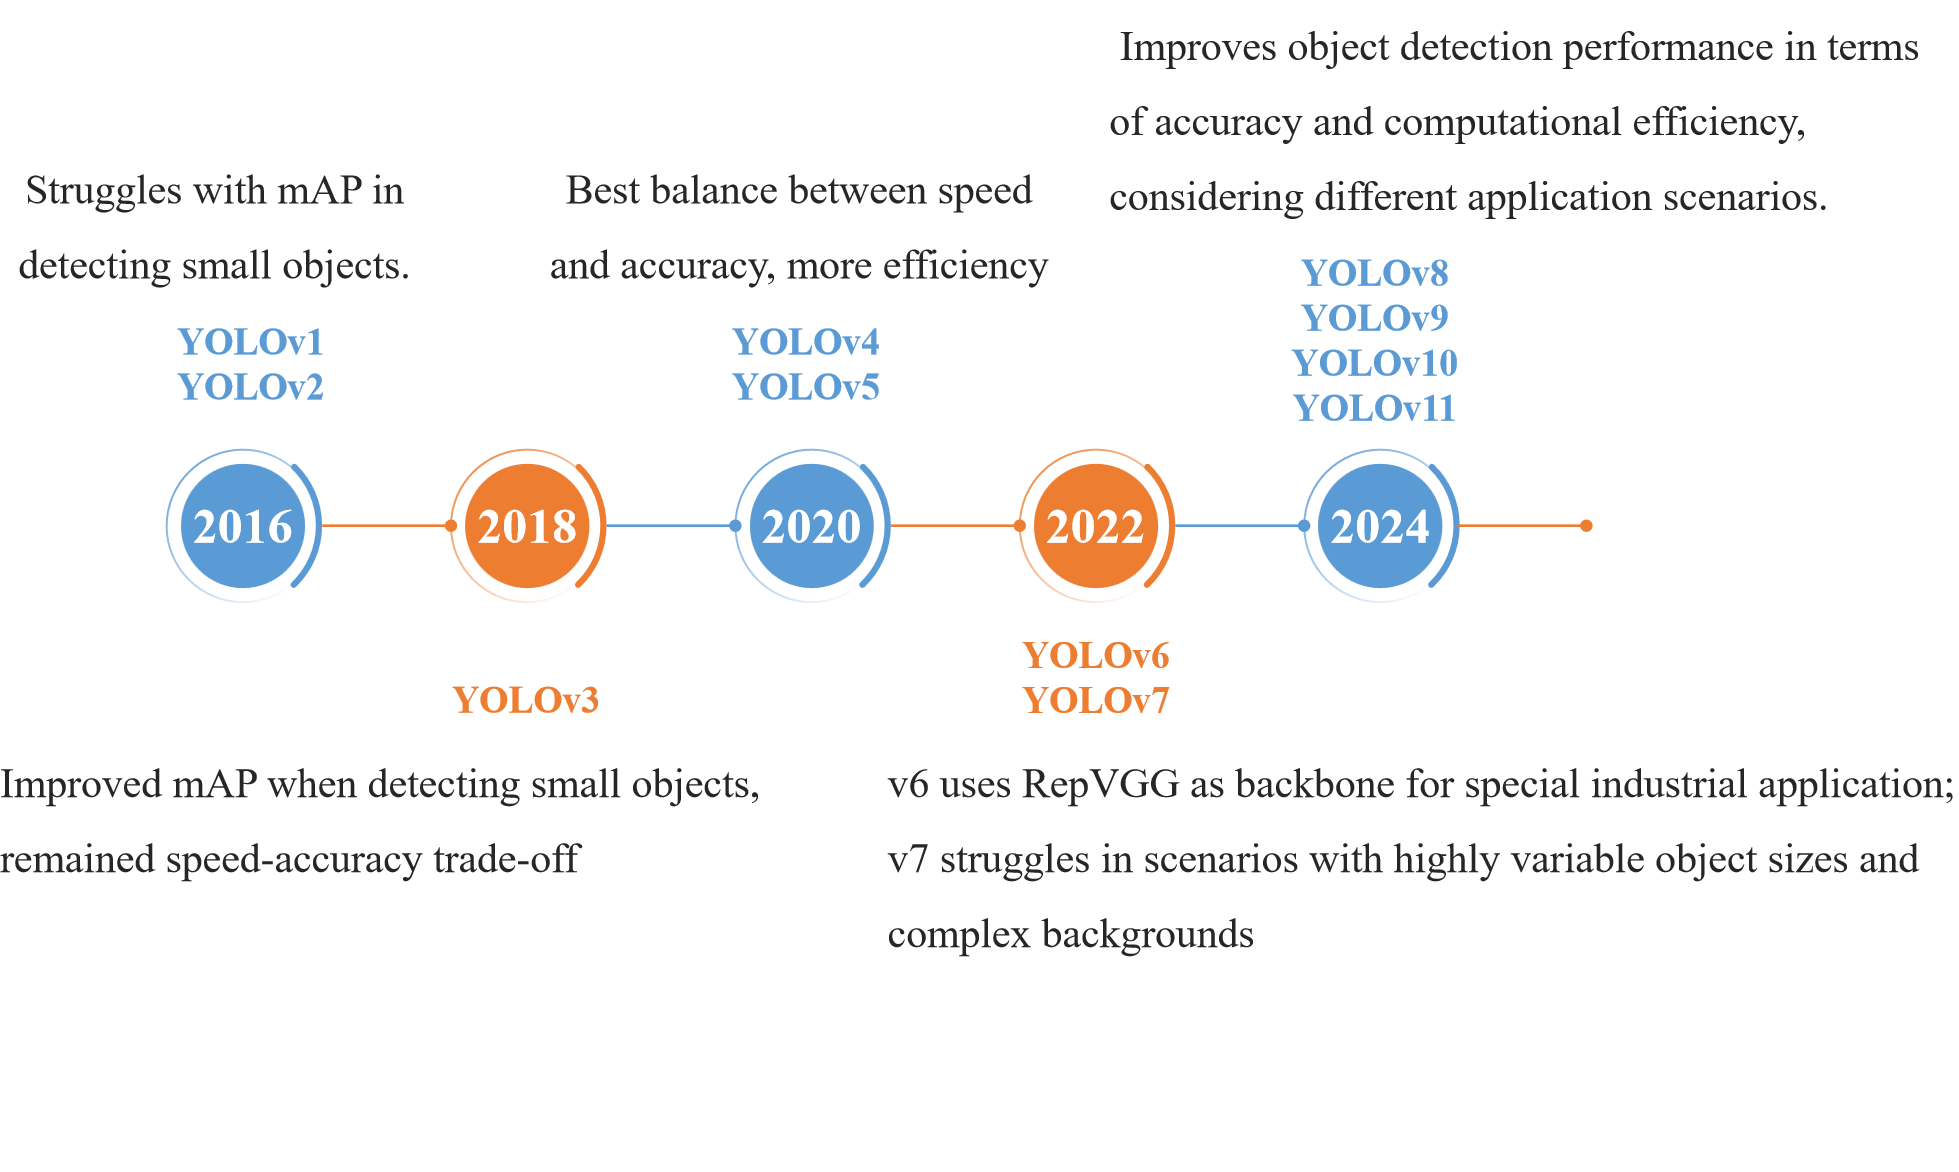
\includegraphics[width=0.5\textwidth]{fig_yolo.png}
\caption{The YOLO Series Roadmap.}
\label{fig:yolo}
\end{figure}

In recent years, YOLOv3~\cite{redmon2018yolov3}, YOLOv4~\cite{bochkovskiy2020yolov4}, and YOLOv5 have emerged as the dominant choices for fruit-picking applications. YOLOv3 introduced the Darknet-53 backbone and multi-scale prediction, enabling more accurate detection of small fruits obscured by leaves. YOLOv4 further optimized performance by integrating techniques like Cross Stage Partial Darknet53 (CSPDarknet53) and Complete Intersection over Union (CIoU) loss, striking a balance between speed and accuracy suitable for real-time robotic operations. 
Subsequent versions, such as YOLOv5 and YOLOv8, incorporated optimizations like CSPNet backbones and auto-learning bounding boxes, achieving frame rates over 100 FPS on edge devices. In fruit-picking contexts, YOLOv8 has been adapted for multi-class detection, distinguishing ripe from unripe fruits with mAP values around 0.92, making it ideal for mobile robots navigating orchards. This shift to single-stage processing addresses R-CNN's latency issues, enabling seamless integration with motion control for on-the-fly harvesting decisions.
%YOLOv5, initially released as an open-source project by Ultralytics (without a traditional academic paper in the same format as others) has a modular design with customizable scales (e.g., n, s, m, l, x) allows researchers to tailor the model for different hardware constraints in the orchard, from edge devices on robotic arms to onboard GPUs. However, their reliance on traditional feature extraction and post-processing limits performance in highly occluded or low-light environments common in orchards.
Conversely, YOLOv6~\cite{li2022yolov6} and YOLOv7~\cite{wang2023yolov7} encounter difficulties when adapting to direct fruit picking. YOLOv6 has been designed with industrial assembly line scenarios in mind. It employs a Re-parameterized VGG (RepVGG) model to facilitate inference-time acceleration.  However, it encounters challenges when confronted with fruits of irregular poses and complex backgrounds. 
Despite its advanced Extended-efficient-layer aggregation networks (ELAN) architecture and  "bag-of-freebies" trainable, YOLOv7 demands substantial computational resources which conflicts with the power constraints of most fruit-picking robots. It is evident that both of these systems necessitate optimisations that are specific to the agricultural domain. 

The most recent iterations of YOLO (v8-v11)~\cite{yaseen2024yolov9, wang2024yolov10, khanam2410yolov11}, present promising directions but remain in the exploratory phase for fruit-picking. They demonstrate potential but remain in the exploratory stage. The YOLOv8 model facilitates multitasking capabilities, encompassing operations such as object detection, instance segmentation, and classification, thereby enabling the concurrent identification of fruit ripeness. YOLOv9's Generalized Efficient Layer Aggregation Network (GELAN) and Programmable Gradient Information (PGI) enhance feature extraction across fruit scales, potentially improving detection of clustered or differently-sized fruits. It is evident that YOLOv10's NMS has the capacity to reduce inference latency. YOLOv11's Spatial Pyramid Pooling Fast (SPPF) and Convolutional Block with Parallel Spatial Attention (C2PSA) components improve attention to occluded fruits, albeit with an attendant increase in task complexity.
%Currently, most research on YOLOv8 - v11 focuses on general object detection in autonomous driving, surveillance, and industrial inspection, where abundant computational resources and controlled data distributions facilitate rapid model development. In fruit picking, although initial studies have demonstrated improved detection rates for specific fruit types, challenges persist. These include handling diverse weather conditions, adapting to varying fruit growth patterns, and ensuring reliable operation on resource - constrained robotic platforms. As such, while YOLOv8 - v11 represent the cutting - edge of object - detection technology, their full integration into fruit - picking systems requires further optimization, validation across multiple crop types, and real - world deployment testing, solidifying their status as a critical research frontier in agricultural robotics.

%The YOLO family of algorithms represents a critical advancement in real-time object detection, with broad adoption in agricultural robotics, particularly for fruit-picking applications. The principal advantage of YOLO is its speed: the framework processes entire images in a single neural network pass, predicting bounding boxes and class probabilities concurrently. This attribute makes it exceptionally well-suited for scenarios requiring rapid and reliable detection, such as autonomous harvesting.
%The evolution of the YOLO series has seen continual enhancement in detection performance, model efficiency, and adaptability to complex environments. YOLOv3 introduced multi-scale feature detection, improving the identification of small and variably sized fruit objects within dense canopies, a frequent challenge in orchard environments. Further, YOLOv4 delivered improvements in accuracy and computational speed by integrating architectural advancements such as the CSPDarknet53 backbone, PANet path aggregation, and optimized anchor box selection. While YOLOv5 is not an official release from the original authors, it has gained substantial traction in the research community due to its user-friendly implementation, fast training times, and lightweight architecture, making it a popular choice for deployment on resource-constrained agricultural platforms.


Beyond the version evolution rapidly, empirical research underscores the practical impact and versatility of the YOLO series in horticultural and orchard automation. For example, Liu et al.~\cite{liu2020yolo} proposed an improved YOLOv3 architecture (YOLO-Tomato) tailored for robust tomato detection under variable lighting and occlusion, demonstrating high precision and field applicability. Lawal~\cite{lawal2021tomato} presented further enhancements to YOLOv3 for tomato detection, offering improved accuracy and operational speed that meet real-time harvesting requirements.
Complex fruit environments often require specialized modifications. Gai et al.~\cite{gai2023detection} advanced detection for cherries by integrating DenseNet modules into an improved YOLOv4 model and introducing a circular bounding box approach, significantly boosting performance under challenging lighting and occlusion. Similarly, Kuznetsova et al.~\cite{kuznetsova2020using} demonstrated that pre- and post-processing strategies improve YOLOv3 performance for apples in natural orchards by effectively addressing issues of varying lighting and object obstruction.
Lightweight models within this family are particularly important for real-time deployment. Magalhães et al.~\cite{magalhaes2021evaluating} systematically evaluated SSD MobileNet v2 and YOLOv4 Tiny for greenhouse tomato detection, confirming their suitability for integration with autonomous harvesting machinery and for mitigating the costs associated with manual agricultural labor. Li et al.~\cite{li2021real} further modified the YOLOv4-Tiny model (YOLO-Grape) for grape detection by incorporating depthwise separable convolutions, attention mechanisms, and the Mish activation function, achieving an F1-score of 90.47\% and real-time detection speeds suitable for orchards with complex backgrounds.
Several studies have explored integrating these detection algorithms with complementary vision and robotic technologies. Tang et al.~\cite{tang2023fruit} enhanced the YOLOv4-Tiny framework with k-means++ clustering and additional convolutional layers, utilizing binocular stereo vision to support precise fruit localization in orchards. Sozzi et al.~\cite{sozzi2022automatic} compared the efficacy of multiple YOLO models for white grape detection, demonstrating that YOLOv4 and YOLOv5 deliver superior accuracy and speed, which is essential for vineyard yield estimation and management.
Earlier breakthroughs include Bresilla et al.~\cite{bresilla2019single}, who applied a modified YOLO architecture for real-time detection of apples and pears within tree canopies, achieving accuracy rates above 90\% at over 20 frames per second. This work confirmed the feasibility of deploying DL-based detection for efficient automated harvesting. Jun et al.~\cite{jun2021towards} developed a tomato-harvesting robot that combined the YOLOv3 detection model with RGB-D sensors for three-dimensional localization, paired with a specialized end-effector, resulting in a detection precision of 95\% and efficient harvest cycles in laboratory experiments.

Overall, the YOLO series has significantly contributed to real-time object detection and localization in agricultural robotics. The adaptations and continual improvements across YOLOv3, YOLOv4, and YOLOv5 have addressed core challenges such as detecting small or occluded fruit, optimizing inference for dense foliage, and maintaining computational efficiency in the field. Table~\ref{tab:yolo-based} provides a comparative overview of different YOLO versions, illustrating the specific enhancements that advance their suitability for diverse, real-world agricultural environments. These developments collectively promote both the reliability and scalability of autonomous fruit-picking systems.


\begin{table*}[htbp]
	\centering
	\footnotesize 
	\caption{Summary of YOLO Family Approaches for Fruit Detection since 2019 (part 1)} 
	\label{tab:yolo-based}
	\begin{tabular}{@{}p{0.025\textwidth}p{0.094\textwidth}p{0.084\textwidth}p{0.15\textwidth}p{0.25\textwidth}p{0.26\textwidth}@{}}
	\toprule
	\textbf{Ref. \newline /Year} & \textbf{Fruit \newline /Orchard} & \textbf{Model} & \textbf{Key Focus} & \textbf{Strengths} & \textbf{Limitations} \\ \midrule
	
	\cite{liu2020yolo} \newline 2020 & Tomato \newline Greenhouse & YOLO-Tomato (YOLOv3 + dense architecture) & Circular bounding box for occlusion handling & - AP=96.4\%, F1=93.91\% \newline - Detection time: 54 ms/image \newline - Sunlight recall: 93.22\%; shading recall: 92.94\% & - Severe occlusion recall (90.10\%) 4.48\% lower than slight occlusion \newline - Unripe tomato precision (91.2\%) 3.5\% lower than ripe \newline - Requires 160 epochs for convergence \\ \midrule
	\cite{lawal2021tomato} \newline 2021 & Tomato \newline Greenhouse & YOLO-Tomato-A/B/C (modified YOLOv3) & SPP and Mish activation for small targets & - YOLO-Tomato-C: AP=99.5\%, 52 ms/image \newline - F1-score: 97.9\% (vs. 93.9\% for baseline YOLOv3) \newline - 2.1\% higher AP than YOLOv4 on 0.25 ratio images & - Model size increases by 15\% with SPP \newline - Training requires 50,000 iterations (about 12 hours) \newline - Green tomato precision drops by 3.1\% vs. red \\ \midrule
	\cite{gai2023detection} \newline 2023 & Cherry \newline Outdoor orchard & YOLOv4-dense & DenseNet backbone + circular bounding box & - mAP=0.15 higher than YOLOv4 \newline - F1=0.947, IOU=0.856 \newline - Ripe cherry recall: 95.8\% (vs. 94.9\% for unripe) & - Detection time: 0.467 s/image (1.13× slower than YOLOv4) \newline - Severe occlusion reduces F1 by 10.6\% \newline - Requires 150 epochs for convergence \\ \midrule
	\cite{kuznetsova2020using} \newline 2020 & Apple \newline Outdoor orchard & YOLOv3 + pre/post-processing & Pre-processing (CLAHE, median filter) for backlight & - Precision=92.2\%, recall=90.8\% \newline - Detection time: 19 ms/fruit \newline - FP rate=7.8\%, FN rate=9.2\% & - Green apple recall (83.7\%) 10.1\% lower than red apples \newline - Far-view canopy images require 9-region splitting \newline - Backlight reduces precision by 5.3\% without pre-processing \\ \midrule
	\cite{magalhaes2021evaluating} \newline 2021 & Tomato \newline Greenhouse & SSD (MobileNet v2/Inception v2), YOLOv4-tiny & TPU-compatible models for real-time detection & - SSD MobileNet v2: F1=66.15\%, 16.44 ms/image \newline - YOLOv4-tiny: 5 ms/image, F1=63.78\% \newline - mAP=51.46\% (SSD MobileNet v2 vs. 48.54\% YOLOv4-tiny) & - Green tomato detection F1 (58.2\%) 8.0\% lower than reddish \newline - Overlapping fruits reduce precision by 12.3\% \newline - SSD ResNet 101 shows 15.2\% lower F1 than MobileNet v2 \\ \midrule
	\cite{li2021real} \newline 2021 & Table grape \newline Outdoor vineyard & YOLO-Grape (improved YOLOv4-tiny) & Depthwise separable conv and Soft-NMS for occlusion & - mAP=91.08\%, F1=90.47\% \newline - Detection speed: 81 FPS (12.34 ms/image) \newline - 6.69\% higher mAP than YOLOv4-tiny & - Severe occlusion reduces F1 by 6.5\% \newline - Green grape precision (89.0\%) 3.2\% lower than purple-black \newline - Model size (30 MB) 33\% larger than YOLOv4-tiny \\ \midrule
	\cite{tang2023fruit} \newline 2023 & Camellia oleifera \newline Outdoor orchard & YOLO-Oleifera (improved YOLOv4-tiny) & K-means++ clustering and binocular positioning & - AP=92.07\%, detection time=31 ms/image \newline - Positioning error: 23.568±7.420 mm (sunlight) \newline - Model size=29 MB (smaller than YOLOv5-s by 45\%) & - Severe occlusion reduces recall by 5.05\% \newline - Shading conditions increase positioning error by 0.044 mm \newline - Requires stereo matching for 3D localization \\ \midrule
	\cite{sozzi2022automatic} \newline 2022 & White grape \newline Outdoor vineyard & YOLOv3, YOLOv4, YOLOv5 (x/s/tiny) & Real-time bunch detection under variable illumination & - YOLOv4: F1=0.77, 32 FPS; YOLOv5x: F1=0.76, 31 FPS \newline - YOLOv4-tiny: 196 FPS with F1=0.69 \newline - Bunch count error: 13.3\% per vine & - YOLOv3 affected by FP-FN compensation (RMSE=2.63) \newline - Detection accuracy drops 8\% under direct sunlight \newline - Tiny models show 8-10\% lower F1 than full versions \\ \midrule
	\cite{bresilla2019single} \newline 2019 & Apple, Pear \newline Outdoor orchard & Modified YOLOv2 (M1-M3) & Single-shot detection with splitter/joiner blocks & - M3+AS model: F1=0.90, IoU=0.64 \newline - 20 FPS on NVIDIA 960M \newline - Transfer learning: pear F1=0.87 with 50 images & - M1 model: 5 FPS (too slow for real-time) \newline - Synthetic images improve IoU by only 3\% \newline - Occlusion reduces detection by 5-15\% \\ \midrule
	\cite{jun2021towards} \newline 2021 & Tomato \newline Greenhouse & YOLOv3 + custom end-effector & 3D perception + tractional cutting unit (TCU) & - Precision=0.80, recall=0.91, mAP=0.9082 \newline - TCU cuts stems up to 6 mm diameter \newline - Total cycle time=5.87 s & - Cluster harvest success drops from 100\% (1 fruit) to 41.67\% (4 fruits) \newline - Scissor tips cause 15\% damage to adjacent fruits \newline - Path planning fails for 8\% of target poses \\ \midrule
	\cite{yu2020real} \newline 2020 & Strawberry \newline Ridge-planting greenhouse & R-YOLO (rotated YOLOv3) & Rotated bounding boxes for picking point localization & - Precision=94.43\%, recall=93.46\% \newline - 18 FPS on Jetson TX2 \newline - Harvest success rate=84.35\% (vs. 72.74\% for YOLOv3) & - Unripe fruit F1 (91.11\%) 4.7\% lower than ripe \newline - Curved stems cause ±2 mm localization error \newline - Malformed fruits increase error to 4 mm \\ \midrule

	\end{tabular}
\end{table*}

\begin{table*}[htbp]
	\centering
	\footnotesize 
	\caption{Summary of YOLO Family Approaches for Fruit-Picking since 2019 (part 2)} 
	\addtocounter{table}{-1}
	\begin{tabular}{@{}p{0.025\textwidth}p{0.094\textwidth}p{0.084\textwidth}p{0.15\textwidth}p{0.25\textwidth}p{0.26\textwidth}@{}}
	\toprule
	\textbf{Ref. \newline /Year} & \textbf{Fruit \newline /Orchard} & \textbf{Model} & \textbf{Key Focus} & \textbf{Strengths} & \textbf{Limitations} \\ \midrule
	 \cite{yu2024object} \newline 2024 & Citrus \newline Natural orchard & YOLOv5-citrus & Multi-channel information fusion + state classification & - 2.8\% higher in mAP than original YOLOv5 \newline - Precision 3.7\% higher than original YOLOv5 \newline - 3D positioning error: (1.97 mm, 0.36 mm, 9.63 mm) & - Training requires 4200 images (700 original + 3500 augmented) \newline - Severe occlusion may misclassify "difficult-to-pick" fruits \newline - Slightly slower inference due to added modules (no specific speed given) \\ \midrule
	\cite{ZHOU2024110} \newline 2024 & Camellia oleifera \newline Outdoor orchard & YOLOv8x + binocular vision & 3D positioning of grabbing points via transfer learning & - mAP$_{50}$=0.96 (full dataset); 0.95 with 200 samples (transfer learning) \newline - 3D coordinate error <2.1 cm on all axes \newline - 5 FPS on Jetson Orin & - Severe branch occlusion reduces recall by 5.05\% \newline - Shading increases positioning error by 0.044 mm \newline - Requires 150 epochs for convergence \\ \midrule
	\cite{ZHANG2024108780} \newline 2024 & Tree trunks, person, mast \newline Natural orchard & Improved YOLOv5 & GhostNet V2 + SIoU + Coordinate Attention (CA) & - mAP=97.1\%, 198.2 ms/image \newline - Model size reduced by 43.6\% (7.7 MB) \newline - DBSCAN clustering accuracy=89.2\% & - Supporter AP (94.7\%) 3.2\% lower than tree trunks \newline - Overexposure increases false negatives by 5\% \newline - Requires 350 epochs for convergence \\ \midrule
	\cite{ZHANG2024108836} \newline 2024 & Citrus \newline Complex orchard & MFAF-YOLO (modified YOLOv5s) & Multi-scale feature adaptive fusion + K-means++ anchor boxes & - mAP=90.2\%, FPS=86.2 \newline - First priority AP=93.2\%, Second priority AP=87.3\% \newline - Model size=10.7 MB (26.2\% smaller than YOLOv5s) & - Dense citrus clusters reduce recall by 8\% \newline - Foggy conditions decrease mAP by 2.1\% \newline - Dual detection heads miss 0.8\% of large fruits \\ \midrule
	\cite{LU2024108721} \newline 2024 & Citrus \newline Complex orchard & MFAF-YOLO (extended) & Res-Attn module + priority-based detection & - Robust to 7 augmentation types (fog, noise, etc.) \newline - Field test success rate=91\% for first priority fruits \newline - 11.6 ms/image inference time & - Immature citrus false detection rate=3.5\% \newline - Stem detection error affects picking precision \newline - MobileNetV3-YOLOv5s is 10\% faster but 4.8\% lower mAP \\ \bottomrule


	\end{tabular}
\end{table*}
	
\iffalse
\begin{table*}[H]
	\centering
	\footnotesize 
	\caption{Summary of YOLO Family Approaches for Fruit-Picking since 2019 (part 2)} 
	\label{tab:yolo-based} 
	\begin{tabular}{p{0.03\linewidth} p{0.03\linewidth} p{0.06\linewidth} p{0.06\linewidth} p{0.12\linewidth} p{0.12\linewidth} p{0.12\linewidth} p{0.28\linewidth}}
	\toprule
	\textbf{Ref.} & \textbf{Year} & \textbf{Fruit Type} & \textbf{Model Type} & \textbf{Main Gap} & \textbf{Performance} & \textbf{Datasets} & \textbf{Key Insights} \\ \midrule
\cite{liu2020yolo}  & 2021 & Tomato & YOLOv3 & Detection across growth stages & Effective in complex environments & Farming environments & Optimized for agricultural applications, real-time capable \\ \midrule
\cite{lawal2021tomato} & 2023 & Tomato & Modified YOLOv3 & Greenhouse environment & SSD MobileNet v2 top performer & Greenhouse dataset & Compares SSD and YOLO models \\ \midrule
\cite{gai2023detection} & 2023 & Cherry & Improved YOLO-v4 & Detection in varying conditions & High AP & Controlled conditions & Enhanced with DenseNet; circular bounding boxes \\ \midrule
\cite{kuznetsova2020using} & 2023 & Apple & YOLOv3 & Pre-/Post-Processing & High efficiency & Orchard dataset & Advanced pre-/post-processing \\ \midrule
\cite{magalhaes2021evaluating} & 2023 & Tomato & YOLO & Greenhouse accuracy & Superior detection & Controlled conditions & Improved accuracy and speed \\ \midrule
\cite{li2021real} & 2023 & Grape & YOLOv4-Tiny & Complex background & F1-score 90.47\% & Vineyard images & Real-time, low computational cost \\ \midrule
\cite{tang2023fruit} & 2023 & Camellia oleifera & YOLOv4-Tiny & Precise positioning & AP 92.07\% & Orchard dataset & Combines DL with stereo vision \\ \midrule
\cite{sozzi2022automatic} & 2023 & Grape & YOLOv3, YOLOv4, YOLOv5 & Bunch detection & Best F1-score 0.77 & Vineyard dataset & Effective in vineyard settings \\ \midrule
\cite{jun2021towards} & 2021 & Tomato & YOLOv3 with RGB-D sensors & Accurate and efficient harvesting in greenhouses & 95\% detection precision; 5.9 seconds per tomato & 770 images from greenhouse environment & Combines 3D perception and a novel end-effector design to enhance efficiency and reduce fruit damage during harvesting. \\ \midrule
\cite{yu2020real} & 2020 & Strawberry & R-YOLO & Localization in narrow spaces & Recognition rate 94.43\%, Recall 93.46\% & Ridge-planting strawberry fields & Utilizes rotated YOLO for precise localization; optimizes real-time performance on embedded systems \\  \midrule
\cite{bresilla2019single}& 2019 & Apple, Pear & Modified YOLO & Real-time detection in complex backgrounds & Over 90\% accuracy, 20+ FPS & Orchard images & Optimizes YOLO for fast, accurate fruit detection suitable for robotic harvesting \\  \midrule
\cite{yu2024object} & 2024 & Citrus & Improved YOLOv5 & Leaf occlusion, overlapping fruits, and variable lighting conditions  &  A high detection precision of 95.83\% and a mAP of 79.68\% & Orchard dataset & Enhanced the YOLOv5 model by introducing receptive field convolutions with full 3D weights (RFCF), addressing the limitations from parameter sharing in traditional convolution operations and thus improving detection accuracy.. \\ \midrule  
\cite{ZHOU2024110} & 2024 & \textit{C. oleifera} & YOLOv8x & 3D positioning for robotic harvesting & mAP50: 0.96 & Annotated \textit{C. oleifera} dataset (1012) & Integration of depth cues with advanced 2D detection delivers sub-centimeter positioning accuracy for harvesting robots. \\ \midrule 
\cite{ZHANG2024108780} & 2024 & Fruit tree trunk & Improved YOLOv5 & Trunk detection for orchard operation robots & mAP=97.1\% & Natural orchard (1354 images) & Hybrid attention modules bolster trunk recognition under variable illumination and occlusion conditions. \\ \midrule  
\cite{ZHANG2024108836} & 2024 & Citrus & MFAF-YOLO & Real-time detection in complex citrus orchards & mAP=90.2\%, AP (First priority): 93.2\%, AP (Second priority): 87.3\% & Real-field citrus images & Multi-frequency attention mechanisms dynamically adapt to different citrus growth stages and environmental conditions. \\ \midrule  
\cite{LU2024108721} & 2024 & Citrus & Yolo-FD & Citrus peel defect and fruit morphology detection & mAP=98.7\%, Morphology Accuracy: 91.42\% & N/A & Dual-branch design enables simultaneous defect detection and morphological analysis for enhanced quality control. \\ \bottomrule
\end{tabular}
\end{table*}
\fi
\subsection{Segmentation Techniques: Enhancing Precision in Complex Environments}
R%ecent advancements in DL have notably improved fruit detection and segmentation, addressing longstanding challenges in agricultural robotics such as varying lighting, occlusion, and complex backgrounds. Through continual development and the adaptation of neural network architectures, segmentation networks now support enhanced autonomy and operational performance in fruit-picking robots.
Transitioning from bounding-box-based detection in YOLO to more granular analysis, semantic and instance segmentation techniques further refine visual perception by classifying pixels and segmenting individual instances. Unlike earlier subsections that focused on detection pipelines, this part emphasizes segmentation's role in enabling robots to assess fruit maturity and plan occlusion-aware paths.

Initial efforts in fruit segmentation largely relied on color, shape, and edge features.
%Building on R-CNN's instance segmentation, YOLO offers complementary single-stage detection for real-time applications. 
For instance, Lu and Sang~\cite{lu2015detecting} developed a technique for detecting citrus fruits under natural light using color properties, contour fragments, and ellipse fitting to robustly segment and identify fruit despite occlusion. 
%Liu et al.~\cite{liu2016method} proposed a two-stage apple segmentation method combining color and positional information to enable accurate night-time detection. 
Lehnert et al.~\cite{lehnert2016sweet} utilized color segmentation and 3D clustering to estimate the pose of sweet peppers, enabling precise robotic grasping with a 6-DOF manipulator. 
Wang et al.~\cite{wang2017robust} enhanced segmentation robustness under variable illumination by combining wavelet-based normalization, Retinex image enhancement, and K-means clustering, thereby improving overall detection accuracy.

With the progress of DL, CNNs and fully convolutional architectures became mainstream. Initial efforts in semantic segmentation utilized models like U-Net, which employs an encoder-decoder architecture for pixel-wise classification, proving effective in segmenting fruit regions from foliage with Intersection over Union (IoU) metrics above 0.80~\cite{ronneberger2015u}. DL progress has since introduced transformer-based models, such as SegFormer, which leverage self-attention mechanisms for better handling of irregular shapes and textures in tropical fruits~\cite{xie2021segformer}. 
%Peng et al.~\cite{peng2018general} improved the SSD model by integrating ResNet-101 with the SSD framework to detect multiple fruit types in open environments. This adaptation resulted in high detection accuracy and efficiency, with an average accuracy of 89.53\% and an F1-score of 96.12\%. 
Barth et al.~\cite{barth2018data} contributed a synthetic dataset approach for semantic segmentation of Capsicum annuum using procedurally modeled imagery, demonstrating significant gains in data augmentation and model generalizability.
%Lin et al.~\cite{lin2019guava} and 
Lin et al.~\cite{lin2020color} advanced the field by using low-cost RGB-D sensors and fully convolutional networks (FCN) for guava detection and 3D pose estimation. These systems delivered high accuracy in fruit segmentation and localization with rapid processing, supporting practical implementation in resource-constrained environments.

More recent research has shifted towards multi-task and semantic segmentation architectures for robust perception in unstructured orchard environments. Kang and Chen~\cite{kang2019fruit, kang2020fruit} introduced the DaSNet and DaSNet-v2 models, employing ResNet backbones and Gated Feature Pyramid Networks for simultaneous detection and semantic segmentation of fruits and branches. Their systems achieved high F1-scores and demonstrated ability to handle complex orchard scenes, providing 3D environmental visualizations critical for autonomous navigation and harvesting. Majeed et al.~\cite{majeed2020deep} applied the SegNet architecture for semantic segmentation of apple tree canopies, facilitating tasks such as trunk, branch, and trellis identification to automate orchard management and training processes.
For specific crop types, 
%Birrell et al.~\cite{birrell2020field} presented Vegebot, a robotic harvester for iceberg lettuce, integrating advanced vision with robotic manipulation to achieve a 91\% localization rate in field conditions. 
Luo et al.~\cite{luo2018vision} developed a vision-based methodology that accurately detects cutting points on grape peduncles, overcoming the occlusion and variability of vineyards, achieving an average accuracy of 88.33\%.
Semantic segmentation with models such as DeepLabV3 and U-Net further refined perception in agricultural robotics. 
%Peng et al.~\cite{peng2020semantic} optimized DeepLabV3 with the Xception65 backbone for litchi branch segmentation, reporting a mean intersection-over-union of 0.765; 
Li et al.~\cite{li2020detection, li2021novel} extended semantic segmentation for litchi and green apples using RGB-D data, ensemble U-Net models, edge structures, and gated convolutions, achieving high accuracy in complex, real-world orchard environments.
%Pereira et al.~\cite{pereira2019deep} focused on the identification of grape plant species via transfer learning and AlexNet, successfully distinguishing visually similar varieties under challenging conditions with test accuracies up to 89.75\%. 
Rahnemoonfar and Sheppard~\cite{rahnemoonfar2017deep} introduced "Deep Count"—a synthetic data-driven fruit counting network, achieving 91\% accuracy, illustrating the value of artificial datasets in overcoming ground truth limitations.
Combining segmentation with contemporary detection algorithms has further improved system robustness. 
%Luo et al.~\cite{luo2016robust} combined AdaBoost and color component analysis for resilient grape detection in unstructured settings. 
Kirk et al.~\cite{kirk2020b} integrated bio-inspired features and the CIELab color space into a RetinaNet model to enhance strawberry detection under variable lighting, achieving superior F1-scores compared to traditional approaches. 
%Peng et al.\cite{peng2018general} and 
Feng et al.~\cite{feng2018} demonstrated that integrating classic image processing (edge detection, color segmentation) with DL yields high accuracy for challenging targets such as cherry tomato bunches.

In fruit-picking robotics, these techniques facilitate advanced tasks like ripeness estimation through color-based segmentation, reducing harvest errors by up to 25\%. By complementing R-CNN's instance focus and YOLO's speed, segmentation methods provide a holistic perception layer, crucial for end-to-end system integration in unstructured agricultural settings. 
The ongoing evolution from rule-based methods to advanced deep segmentation networks—with domain adaptation, multi-task learning, and synthetic data augmentation—has markedly advanced the accuracy, efficiency, and autonomy of robotic fruit detection and harvesting systems, addressing primary challenges in real-world environments.
%The ongoing evolution from rule-based methods to advanced deep segmentation networks—with domain adaptation, multi-task learning, and synthetic data augmentation—has markedly advanced the accuracy, efficiency, and autonomy of robotic fruit detection and harvesting systems. These approaches address the primary challenges of real-world agricultural environments, setting new standards for performance and practical adoption in precision agriculture.

\subsection{Core Performances Metrics of Fruit-Picking}
The practical deployment of fruit-picking robots faces several challenges, focused on the precision, rapidity and reliability as illustrated in Figure~\ref{fig:performance}. Researchers have proposed various solutions to address these challenges.
Fruit picking-point detection in agricultural robotics typically involves identifying where the fruit attaches to the plant, which is crucial for effective and damage-free harvesting. The algorithms used for this purpose often include image segmentation techniques, edge detection, Geometric and Morphological Features, and ML models.
Image Segmentation techniques separate different parts of the plant based on color, texture, or depth information. For example, the stem of sweet peppers can often be distinguished from the fruit and leaves by its distinct color and texture characteristics.
Once the regions of interest (e.g., potential stem areas) are segmented, edge detection algorithms might be applied to outline the precise boundaries of the stem, which can help pinpoint the exact location where the fruit connects to the stem.
Algorithms might analyze detected objects' geometric shapes and morphological features to identify stem-like structures, which could involve detecting elongated, cylindrical shapes typical of stems among the rounded shapes of fruits. Advanced implementations might train ML models, particularly CNNs, on labeled images to learn and accurately predict the location of stems.
\begin{figure}[hbtp]
\centering
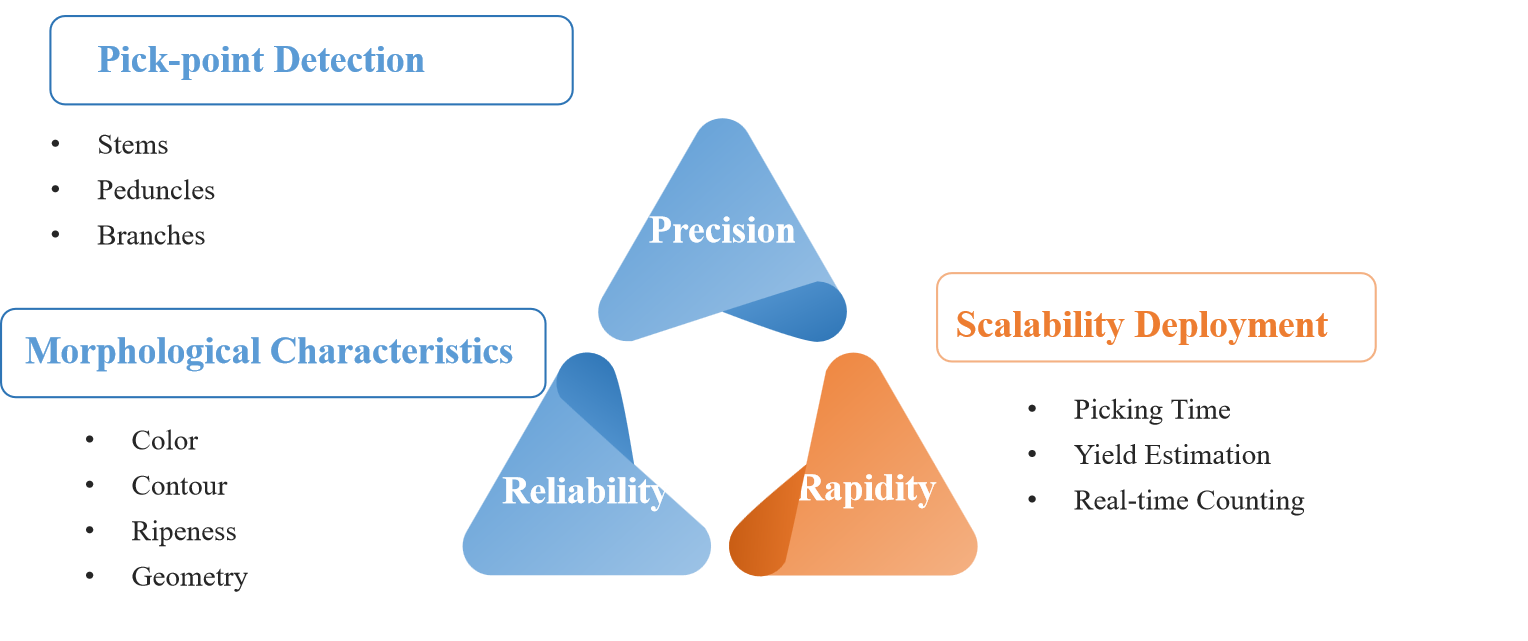
\includegraphics[width=0.57\textwidth]{fig_performance.png}
\caption{The Core Performances of Fruit-Picking.}
\label{fig:performance}
\end{figure}
Accurate pick-point detection is fundamental to the success of autonomous fruit and vegetable harvesting. Progress in this area has focused on identifying critical structural features, such as stems, peduncles, branches, and optimal cutting points, under varying environmental and crop-specific challenges.
Bac et al.~\cite{bac2017performance} enhanced stem detection reliability by incorporating multispectral imaging and artificial lighting, alongside advanced algorithms that exploit both color and textural differences. This method enabled the robotic system to achieve precise cutting with minimal damage to crops, demonstrating the value of sensor fusion and image enhancement in complex plant structures.
In vineyard applications, Mendes et al.~\cite{mendes2016vine} developed ViTruDe, an advanced visual detection system for the robust identification of vine trunks and masts in situations where GPS is unreliable. By employing techniques such as Sobel keypoint detection, Local Binary Pattern (LBP) region descriptors, and SVM classification, the system achieved greater than 95\% accuracy, thereby enabling precise autonomous navigation and further highlighting the potential of vision-based approaches in challenging agricultural terrains.

Detection of fruit peduncles is critical for minimizing crop damage during harvesting. Sa et al.~\cite{sa2017peduncle} proposed a 3D visual detection method utilizing the combined information from RGB-D sensors, incorporating both color and geometry to identify sweet pepper peduncles. The method achieved a detection area under the curve (AUC) of 0.71 for the precision-recall curve and significantly outperformed color-only techniques, validated on a manually annotated dataset for sweet pepper peduncles.
Luo et al.~\cite{luo2018vision} developed a vision-based approach to detect cutting points on peduncles of grape clusters in complex vineyard environments. By addressing the challenges of overlapping fruits and unstructured conditions, their method achieved an average recognition accuracy of 88.33\% and a success rate of 81.66\% for cutting point localization, demonstrating tangible benefits for robotic grape harvesting.
Yu et al.~\cite{yu2020real} addressed the practical need for real-time pick-point localization in strawberry harvesting. Their R-YOLO architecture employs rotated bounding boxes and MobileNet-V1 for lightweight, rapid feature extraction. Operating at 18 frames per second on embedded hardware, the system identifies optimal strawberry picking points in ridge-planting scenarios with a recognition rate exceeding 94\%, substantially improving picking efficiency and accuracy under authentic agricultural conditions.
Pérez-Zavala et al.~\cite{perez2018pattern} presented a robust vision strategy for grape bunch detection using standard RGB cameras under natural illumination. By integrating Histogram of Oriented Gradients (HOG) for shape and LBP for texture extraction with SVM classification, the approach achieved 88.61\% precision and 80.34\% recall, demonstrating adaptability across grape cultivars and lighting variations, thus supporting practical automated viticulture.

%Collectively, these studies illustrate the progressive refinement of pick-point detection approaches, addressing the diverse requirements of crop types, harvesting scenarios, and environmental complexities. Advanced sensor integration, robust machine vision algorithms, and tailored network architectures have fundamentally improved the reliability and safety of autonomous harvesting systems, driving practical deployment in both protected and open-field agriculture.

The deployment of real-time machine vision systems is a pivotal factor driving the automation and efficiency of agricultural harvesting operations. Recent years have seen substantial progress in the development and application of robust computer vision, ML, and DL methods that fulfill the stringent requirements of agricultural environments, delivering reliable, rapid, and scalable solutions for fruit detection, grading, and harvesting.
Goel and Sehgal~\cite{goel2015fuzzy} proposed a fuzzy rule-based classification system for tomato ripeness estimation, leveraging color feature extraction and a decision tree learning algorithm. Their approach enables rapid and accurate classification of tomatoes into six maturity stages (94.29\% accuracy) using images captured under natural light, reducing subjectivity and labor in the ripening assessment process.
Zhao et al.~\cite{zhao2016robust} advanced tomato recognition for low-cost robotic platforms by fusing features from multiple color spaces, employing the Lab* a*-component and YIQ I-component with wavelet transformation to address illumination variability and occlusion. Their system maintained a recognition rate of 93\% in field tests, demonstrating the reliability of feature fusion techniques for robust, real-time detection.
Lin et al.~\cite{lin2019field} developed a real-time citrus detection and localization approach utilizing RGB-D imaging coupled with depth filtering, density clustering, and SVM classification. Achieving an F1 score of 0.9197 under conditions of variable lighting and partial occlusion, this method improved feasibility for automated orchard harvesting.
Wang L L et al.~\cite{lili2017development} engineered a comprehensive robotic system for greenhouse tomato harvesting, integrating a binocular stereo vision module, laser navigation, and four-wheel steering for efficient mobility. The system delivered high recognition accuracy and precise navigation, illustrating the convergence of multi-modal sensing and motion planning to enhance operational efficiency in dense crop environments.

DL and efficient model architectures have significantly upgraded real-time fruit classification capabilities. Xiang et al.~\cite{xiang2019fruit} deployed MobileNetV2, combined with transfer learning, for lightweight, rapid fruit sorting, achieving 85.12\% accuracy on a heterogeneous dataset and demonstrating practical viability for low-power agricultural devices. Altaheri et al.~\cite{altaheri2019date} automated date fruit classification by fine-tuning AlexNet and VGGNet through transfer learning, attaining high classification accuracy and speeds compatible with real-time robotic harvesting in orchard environments.
Mao et al.~\cite{mao2020automatic} proposed a multi-feature fusion cucumber recognition algorithm, combining a Multi-Path CNN and selective color component analysis. Supported by SVM classification, their approach achieved rapid, high-accuracy detection and proved effective in complex, open-field settings, furthering the development of autonomous harvesting systems.
Barth et al.~\cite{barth2016design} presented a modular software framework designed for robust robotic harvesting in dense crop scenarios, integrating eye-in-hand sensing, visual servo control, and scene reconstruction within the Robot Operate System (ROS) ecosystem. Validated on a synthetic sweet-pepper crop, the system displayed adaptability and efficiency for automated operations in high-density vegetation.
Kang et al.~\cite{kang2020real} further advanced real-time operational efficiency by integrating a DL-based detection module (Mobile-DasNet) with PointNet-based grasp estimation in a robotic apple harvesting system. This configuration enabled precise and reliable picking under various environmental conditions, highlighting the practical benefits of deep network architectures in agricultural robotics.

\begin{table*}[htbp]
	\centering
	\footnotesize 
	\caption{Summary of Fruit Detection Approaches by Core Performances Metrics (2015-2024)} 
	\label{tab:performance-metrics} 
	\begin{tabular}{@{}p{1.5cm}p{2.5cm}p{5cm}p{4cm}p{2.5cm}@{}}
	\toprule
	\textbf{Metrics} & \textbf{Key Focus} & \textbf{Strengths} & \textbf{Limitations} & \textbf{References} \\ \midrule
	\textbf{Reliability} & Handling illumination, occlusion, and overlap via color, 3D contour, and shape; improving ripeness recognition & - Color-based methods: 96\% detection rate for ripe tomatoes under varying light \cite{zhao2016detecting}. Contour analysis: 5.27\% relative error for occluded citrus \cite{lu2015detecting}. 3D depth integration: 82\% detection of occluded apples \cite{nguyen2016detection}. Ripeness classification: 94.29\% accuracy for tomatoes \cite{goel2015fuzzy} & - Color sensitivity to extreme backlighting \cite{liu2016method}. Contour ambiguity in dense grape clusters \cite{luo2016robust}. Limited generalization across fruit types \cite{li2021novel} & \cite{nguyen2016detection}, \cite{lu2015detecting}, \cite{liu2016method}, \cite{lin2020color}, \cite{majeed2020deep}, \cite{li2021novel}, \cite{luo2016robust}, \cite{mendes2016vine}, \cite{goel2015fuzzy}, \cite{zhao2016detecting}, \cite{pourdarbani2020automatic}, \cite{zhang2018deep}, \cite{longsheng2015kiwifruit} \\ \midrule
	\textbf{Precision} & Precise cut-point \newline detection (stem/ peduncle), distinguishing similar plants (trunk/ mast), non-destructive picking & - Peduncle detection: AUC=0.71 for sweet peppers \cite{sa2017peduncle}. Cut-point localization: 81.66\% success rate for grapes \cite{luo2018vision}. Non-destructive grasp: Improved handling of thin-skinned fruits \cite{CHEN2024111082}. Pose estimation: 80\% grasping success for sweet peppers \cite{lehnert2016sweet} & - Stem occlusion reduces accuracy in dense canopies \cite{sa2017peduncle}. Difficulty distinguishing similar citrus varieties \cite{lin2020fruit}. High precision requires complex 3D sensors \cite{kusumam20173d} & \cite{kusumam20173d}, \cite{andujar2016using}, \cite{lehnert2016sweet}, \cite{bac2017performance}, \cite{mendes2016vine}, \cite{sa2017peduncle}, \cite{luo2018vision}, \cite{kirk2020b}, \cite{perez2018pattern}, \cite{liu2019mature}, \cite{pourdarbani2020automatic}, \cite{lin2020fruit}, \cite{luo2018vision}, \cite{peng2020semantic}, \cite{CHEN2024111082}\\ \midrule
	\textbf{Rapidity} & Real-time operation, fast picking/counting, scalable yield estimation & - Inference speed: 28 ms/image for apples \cite{kang2020fast}. Picking cycle: 6.5 s/fruit for apples \cite{kang2020real}. Yield estimation: $R^2=0.77$ for almonds \cite{underwood2016mapping}. Real-time classification: <0.01s per date fruit \cite{altaheri2019date} & - Speed-accuracy trade-off (small fruit detection sacrificed) \cite{kang2020fast}. High computational demand limits edge deployment \cite{kang2019fruit}. Dynamic scenes (e.g., wind) increase counting error \cite{PAL2024104567} & \cite{onishi2019automated}, \cite{underwood2016mapping}, \cite{lin2019guava}, \cite{kang2019fruit}, \cite{kang2020fruit}, \cite{lin2019field}, \cite{xiang2019fruit}, \cite{mao2020automatic}, \cite{barth2016design}, \cite{kang2020real}, \cite{altaheri2019date},  \cite{kang2020fast},  \cite{PAL2024104567} \\ \bottomrule

	\end{tabular}
\end{table*}

Accurate recognition of fruit ripeness is critical for optimizing harvest timing, enhancing post-harvest quality, and enabling targeted automation in agricultural robotics. Recent developments have combined DL, machine vision, and hybrid modeling strategies to improve the reliability and efficiency of ripeness classification under real-world conditions.
Zhang et al.~\cite{zhang2018deep} made a substantial contribution to automated ripeness assessment by developing a DL-based classification system for tomato harvesting robots. Their CNN model, supported by data augmentation techniques, classifies tomatoes into distinct ripeness stages with a high accuracy of 91.9\% and provides rapid predictions (less than 0.01 seconds per image). The versatility and speed of this approach enable its extension to a broad range of fruit crops, marking a significant advancement for fully automated harvesting systems.
Furthering this progress, Liu et al.~\cite{liu2019mature} proposed a robust detection algorithm targeting mature tomatoes in greenhouse conditions. The method integrates HOG descriptors and a SVM classifier to process color features, combined with illumination enhancement and false color removal to reduce the impact of complex backgrounds and lighting variations. Their system achieved a recall of 90\%, a precision of 94.41\%, and an F1-score of 92.15\%, demonstrating both accuracy and reliability in challenging growing environments.
Goel and Sehgal~\cite{goel2015fuzzy} addressed the difficulty of subjective ripeness estimation by introducing a Fuzzy Rule-Based Classification System (FRBCS) that utilizes red-green color differences and ratios extracted from RGB imagery. Employing a Mamdani-type fuzzy inference system with rules automatically generated by decision trees, their system accurately classifies tomatoes into six maturity stages, achieving a classification accuracy of 94.29\%. This result underscores the capacity of fuzzy logic to handle the inherent uncertainty in visual ripeness assessment, particularly under variable natural illumination and occlusion.
Beyond tomatoes, Pourdarbani et al.~\cite{pourdarbani2020automatic} demonstrated a hybrid approach combining artificial neural networks and simulated annealing for non-destructive classification of Fuji apple maturity. By fusing the $\alpha^*$ component from the lab color space with NIR spectral data, their system classified apples into four maturity stages with a correct classification rate of 99.62\% for spectral data (535–560 nm) and 93.27\% for color data alone. This method illustrates the effectiveness of combining multispectral and colorimetric data for reliable, real-time maturity assessment in orchard environments.

Reliable fruit detection in complex agricultural environments often relies on extracting and analyzing shape, edge, or contour features, which help address challenges posed by variable lighting, overlapping objects, and background clutter. Recent research has demonstrated the effectiveness of leveraging these features—often in concert with color analysis and ML techniques—for robust classification and localization in automated harvesting systems.
Zhao et al.~\cite{zhao2016detecting} significantly advanced tomato detection in greenhouse settings by combining AdaBoost classifiers with color information. Their method utilizes Haar-like features to capture shape characteristics and refines detections using post-processing color analysis, resulting in a detection accuracy exceeding 96\%. This integration of shape-based ML and color metrics effectively reduces false negatives and exemplifies the value of sophisticated feature fusion in agricultural vision systems.
Focusing on contour information,
Longsheng et al.~\cite{longsheng2015kiwifruit} addressed the challenge of nighttime kiwifruit detection by integrating artificial lighting with a canopy-mounted RGB camera. Their image processing pipeline, which incorporates an R-G color model alongside Canny edge detection, achieved an 88.3\% success rate for fruit detection under low-light conditions. By overcoming the limitations imposed by natural lighting, this method extends the operational hours and flexibility of robotic harvesting platforms.

This detailed tabulation of learning-based approaches in Table \ref{tab:performance-metrics} offers a clear and structured view of the advancements in fruit detection technologies, helping researchers and practitioners to identify trends, evaluate different methodologies, and understand the progress made in addressing various challenges in the field.

\section{Advances in Motion Control for Fruit-Picking Robotics}
Motion control is a pivotal aspect of fruit-picking robots, essential for ensuring precise and efficient operations in complex agricultural environments. Researchers have developed various advanced algorithms to address the challenges of path planning, obstacle avoidance, and adaptive motion control~\cite{Ahmad:2023_bnb, Loganathan:2024_hho_avoa, Teo:2020, Arrouch:2022b, 10746490}.

\subsection{Algorithmic Path Planning and Obstacle Avoidance in Robotic Fruit Harvesting}
Path planning, a crucial element in the smooth navigation of autonomous robots while avoiding obstacles, is of paramount importance in the field of robotics~\cite {Leong:2024_review}. Key algorithms in this area include A-star (A*) Algorithm, RRT, Dijkstra's Algorithm, and advanced DDPG algorithm~\cite{Loganathan:2023_amr}.
% and  Deep Deterministic Policy Gradient.

The A* algorithm, known for its efficiency in finding the shortest path from a start node to a target node while avoiding obstacles, is a reliable choice for grid-based environments. It combines uniform-cost and greedy best-first search features by using a heuristic to estimate the cost from a node to the goal. The primary equation for A* is:
\begin{equation}
f(n) = g(n) + h(n)
\label{eq:astar}
\end{equation}

Where:
$f(n)$ is the total cost of the node, 
$g(n)$ is the cost from the start node to $n$, 
$h(n)$ is a heuristic that estimates the cost from $n$ to the goal.

The bi-directional Rapidly-exploring Random Tree (Bi-RRT) variant, known for its efficiency in navigating dense obstacle environments, is particularly relevant for applications in agricultural settings like sweet pepper harvesting~\cite {bac2016analysis}. The bi-directional version works simultaneously from both the start and the goal, enhancing its efficiency. 
The Bi-RRT algorithm is a popular path planning algorithm used in robotics to efficiently navigate high-dimensional spaces. It operates by simultaneously growing two trees, one from the start position and another from the goal position until they meet to form a complete path.
The RRT algorithm is designed to explore large, high-dimensional spaces quickly by expanding nodes randomly, ensuring coverage of the search space~\cite{lavalle1998rapidly}.
By growing trees from both the start and goal positions, Bi-RRT can find paths more quickly and efficiently than single-tree RRT, especially in complex environments with many obstacles.
After finding a collision-free path, the Bi-RRT algorithm often includes a path-smoothing step to refine the trajectory, making it more suitable for practical use in robotic applications.
%Relevance to Robotic Harvesting:
In the context of sweet-pepper harvesting, the Bi-RRT algorithm stands out for its adaptability to the dynamic and unstructured nature of agricultural environments. It efficiently navigates through dense foliage and obstacles typical in greenhouse settings, finding feasible paths for the robotic manipulator. The bidirectional approach reduces the time needed to find a valid path, enhancing the overall efficiency of the harvesting process.
The fundamental step involves:

%\subsection*{1. Distance Metric}
The distance metric \( d \) is used to find the nearest node in the tree to a given point \( x \):
\begin{equation}
d(x_1, x_2) = \| x_1 - x_2 \|
\end{equation}
where \( \| \cdot \| \) denotes the Euclidean distance.

%\subsection*{2. Node Expansion}
A new node \( x_{\text{new}} \) is generated by moving from the nearest node \( x_{\text{nearest}} \) towards the random sample \( x_{\text{rand}} \) by a step size \( \epsilon \):
\begin{equation}
x_{\text{new}} = x_{\text{nearest}} + \epsilon \frac{x_{\text{rand}} - x_{\text{nearest}}}{\| x_{\text{rand}} - x_{\text{nearest}} \|}
\end{equation}

%\subsection*{3. Collision Check}
The path between \( x_{\text{nearest}} \) and \( x_{\text{new}} \) must be checked for collisions with obstacles. This is typically done using a collision detection function \( \text{isCollisionFree}(x_{\text{nearest}}, x_{\text{new}}) \):
\begin{equation}
\text{isCollisionFree}(x_{\text{nearest}}, x_{\text{new}})
\end{equation}

%\subsection*{4. Tree Growing}
The tree is grown by adding the new node \( x_{\text{new}} \) if it is collision-free:
\begin{equation}
\text{Tree} \leftarrow \text{Tree} \cup \{x_{\text{new}}\}
\end{equation}

%\subsection*{5. Path Smoothing}
After a path is found, it can be smoothed by checking and directly connecting non-adjacent nodes on the path, removing intermediate nodes if the direct connection is collision-free:
\begin{equation}
\text{isCollisionFree}(x_i, x_j) \quad \text{for} \quad x_i, x_j \in \text{Path}
\end{equation}

Dijkstra’s Algorithm is commonly used in structured environments like orchards or greenhouses where the layout allows for fixed route planning~\cite{silwal2017design, dijkstra1959note}. It is used to find the shortest paths from a source node to all other nodes in the graph. The update step in Dijkstra's algorithm is:
\begin{equation}
\begin{aligned}
\text{for each } v \text{ adjacent to } u: \\
\text{if } \text{dist}[u] + \text{length}(u, v) < \text{dist}[v] \\
\text{then } \text{dist}[v] = \text{dist}[u] + \text{length}(u, v)
\end{aligned}
\label{eq:dijkstra}
\end{equation}
where $u$ is the node currently being considered, $v$ is a node adjacent to $u$, $dist[]$ stores the shortest distance from the source to each vertex, $length(u,v)$ is the edge weight between $u$ and $v$.

Collision avoidance is integral to robotic operations, ensuring the safety of the robot and its environment. Algorithms like Vector Field Histogram (VFH), Dynamic-Window Approach (DWA), and Artificial Potential Fields are designed to guide the robot around obstacles, providing a secure operating environment. 
VFH utilizes a polar histogram grid as a statistical representation of the surroundings, calculating the best direction to move without colliding with any obstacles \cite{silwal2017design}. The key equation for VFH is~\cite{borenstein1991vfh}:
\begin{equation}
m(i) = \begin{cases} 
1 & \text{if } \sum_{j=-k}^k h(i+j) > T \\
0 & \text{otherwise} 
\end{cases}
\label{eq:vfh}
\end{equation}
Where $m(i)$ is the masked polar histogram indicating the presence of an obstacle in the direction $i$,
$h(i)$ is the original polar histogram value at direction $i$, $k$ is the smoothing parameter, $T$ is the threshold determining obstacle presence.

DWA algorithm considers the robot's velocity and heading to predict a set of reachable velocities that avoid collisions~\cite{sepulveda2020robotic}.   The velocity command $(v,\omega)$ is selected by the following optimization~\cite{fox1997dynamic}:
\begin{equation}
(v^*, \omega^*) = \arg \max_{(v, \omega) \in V_s} [ \alpha \cdot \text{heading}(v, \omega) + \beta \cdot \text{dist}(v, \omega) + \gamma \cdot \text{vel}(v, \omega) ]
\label{eq:dwa}
\end{equation}
Where $V_s$ is the set of admissible velocities considering robot dynamics and collision avoidance, $heading(v, \omega)$, $dist(v, \omega)$, and $vel(v, \omega)$ are the cost functions for heading towards the target, distance to the closest obstacle, and forward velocity, respectively. $\alpha$, $\beta$, $\gamma$ are the weights for each cost function.

Artificial potential fields are utilized in various robotic applications, including those in the agricultural sector, to guide robots around obstacles by simulating attractive and repulsive forces~\cite{ling2019dual}. The equation for the Artificial Potential Fields method
\begin{equation}
U_{\text{total}} = U_{\text{attr}} + U_{\text{rep}}
\label{eq:potentialfields}
\end{equation}
where $U_{total}$ is the total potential field, $U_{attr}$ is the attractive potential towards the goal. $U_{rep}$ is the repulsive potential from obstacles.

Innovations in motion control focus on adaptability and efficiency. Recent developments focus on integrating these established algorithms with new, innovative approaches like learning-based approaches and hybrid systems. Reinforcement learning and recurrent neural networks are increasingly combined with traditional path planning algorithms like  DDPG to enhance adaptability and efficiency in dynamic environments, as demonstrated in guava orchards~\cite{lin2021collision}.
The DDPG algorithm is popular for dealing with continuous action spaces, typical in robotics~\cite{lillicrap2015continuous}. It is an actor-critic algorithm that merges ideas from Deep Q-Network (DQN) and deterministic policy gradients, learning policies efficiently in high-dimensional, continuous action spaces.
Integrating different algorithms to leverage their strengths enhances path planning and collision avoidance, as seen in using advanced motion planning algorithms in sweet pepper harvesting~\cite{lehnert2017autonomous}.
% \cite{BioInspiredAlgorithmsReference}.

%DDPG algorithm is increasingly popular in robotic path planning, mainly when dealing with continuous action spaces, which are typical in robotics \cite{lillicrap2015continuous}. DDPG is an actor-critic algorithm that merges ideas from DQN (Deep Q-Network) and deterministic policy gradients. It is well-suited for environments with high-dimensional, continuous action spaces.
DDPG is notable for its ability to learn policies efficiently in high-dimensional, continuous action spaces, making it ideal for robotic applications where precise, continuous control is required. The algorithm consists of two main components: an actor that proposes actions given the current state and a critic that evaluates the action by computing the value function.
DDPG has been successfully applied in various robotic path planning contexts, such as navigating complex environments where traditional algorithms struggle with real-time efficiency and adaptability. For instance, in collision-free path planning, DDPG can optimize a robot's trajectory in a dynamic environment, learning to avoid obstacles while minimizing path length and time.
The critic network updates its weights by minimizing the loss function based on the temporal difference (TD) error. The loss function \( L \) is defined as:
\begin{equation}
L = \frac{1}{N} \sum_i \left(y_i - Q(s_i, a_i | \theta^Q)\right)^2
\end{equation}
where \( y_i = r_i + \gamma Q'(s_{i+1}, \mu'(s_{i+1} | \theta^{\mu'}) | \theta^{Q'}) \) is the target value, calculated using the target networks, \( Q' \) and \( \mu' \) are the target critic and actor networks, \( \theta^Q \) and \( \theta^{\mu} \) are the parameters of the critic and actor networks, \( \gamma \) is the discount factor, and \( N \) is the number of samples.

%\subsection*{Actor Update}
The actor network updates its policy by using the policy gradient:
\begin{equation}
\nabla_{\theta^\mu} J \approx \frac{1}{N} \sum_i \nabla_a Q(s, a | \theta^Q)|_{s=s_i, a=\mu(s_i)} \nabla_{\theta^\mu} \mu(s | \theta^\mu)|_{s_i}
\end{equation}
This gradient indicates changing the actor's parameters to increase the expected reward.

%\subsection*{Adding Noise for Exploration}
Exploration is essential for effective learning in continuous action spaces. Noise is added to the actor's output:
\begin{equation}
a_t = \mu(s_t|\theta^\mu) + \epsilon, \quad \epsilon \sim \text{Noise process}
\end{equation}
where \( \epsilon \) often comes from an Ornstein-Uhlenbeck process, providing temporally correlated exploration beneficial in physical control problems.

\subsection{Advances in Motion Planning and Control for Robotic Fruit Harvesting}
Motion planning in robotic harvesting involves determining the path the robot’s end-effector (e.g., a gripper or cutting tool) should take to reach, grasp, and sever the fruit from the plant. This process is crucial for efficient and precise harvesting while avoiding damage to the fruit and the plant. The studies summarized in Table \ref{tab:path-planning-based} highlight various approaches and challenges in robotic path planning for fruit harvesting from 2015 to 2024.

\begin{table*}   
	\centering
	\footnotesize 
	%\addtocounter{table}{-1}
	%\caption{Summary of Learning-Based Approaches for Fruit Detection in 2015-2024(Part 6)} 
	%\label{tab:machinelearning-based} 
	\caption{Summary of Robotic Path Planning for Fruit Harvesting in 2015-2024(part1)} 
	\label{tab:path-planning-based}
	%\begin{tabular}{@{}p{0.5cm} p{0.6cm} p{1.2cm} p{2.4cm} p{2.2cm} p{2.2cm} p{2cm} p{3.1cm}@{}}
	%\begin{tabular}{@{}p{0.4cm}p{0.4cm}p{1.4cm}p{1.4cm}p{2cm}p{2cm}p{2cm}p{4.5cm}@{}}
	%\begin{tabular}{p{0.025\linewidth} p{0.025\linewidth} p{0.055\linewidth} p{0.13\linewidth} p{0.12\linewidth} p{0.12\linewidth} p{0.12\linewidth} p{0.24\linewidth}}
	\begin{tabular}{p{0.025\linewidth} p{0.025\linewidth} p{0.055\linewidth} p{0.16\linewidth} p{0.135\linewidth} p{0.175\linewidth} p{0.255\linewidth}}
	%{@{}p{0.4cm}p{0.4cm}p{1.4cm}p{1.4cm}p{2cm}p{2cm}p{2cm}p{4.5cm}@{}}
\toprule
%\textbf{Ref.} & \textbf{Year} & \textbf{Fruit} & \textbf{Motion Control} & \textbf{Main Challenges} & \textbf{Performance} & \textbf{Field Test} & \textbf{Key Insights} \\ \midrule
\textbf{Ref.} & \textbf{Year} & \textbf{Fruit} & \textbf{Motion Control} & \textbf{Main Challenges} & \textbf{Performance Metrics} & \textbf{Key Insights} \\ \midrule

\cite{silwal2017design} & 2017 & Apple & Seven DOF manipulator with path optimization & Navigating complex orchard environments & 84\% picking success, average cycle time 7.6 s, in commercial orchard & Demonstrates effective path planning and manipulation within a complex, unstructured environment \\ \midrule
\cite{arad2020development} & 2020 & Sweet Pepper & Autonomous navigation and manipulator movement integrated with vision system & Handling variability in greenhouse environment & Cycle time of 24s; 18\%-61\% success rate, in commercial greenhouse & First extensive field test of sweet pepper harvesting robot showing integration of navigation, manipulation, and vision \\ \midrule
\cite{xiong2020autonomous} & 2020 & Strawberry & Dual-arm system with obstacle-separation algorithm & Navigating and operating in polytunnels & 6.1 s manipulation in single-arm mode, in field tests & Demonstrates successful integration of navigation and manipulation in a complex agricultural environment \\ \midrule
\cite{williams2019robotic} & 2019 & Kiwifruit & Dynamic scheduling for multi-arm coordination & Efficient harvesting in commercial orchards & Successful field trials, high efficiency in commercial orchards & Highlights integration of advanced vision and robotic arms for efficient harvesting \\ \midrule
%\cite{mehta2014vision} & 2014 & Citrus & Cooperative visual servo controller with dual-camera system & Precision in cluttered environments & High precision and control in manipulator movement & Effective in real-world tests & Advanced visual servo control system significantly enhances robotic citrus harvesting efficiency \\ \midrule
\cite{xiong2019development} & 2019 & Strawberry & Integrated mobile platform with manual control & Adaptability to positional inaccuracies & Cycle time of 7.5 s; 96.8\% success in isolation, 53.6\% success rate in field& Novel gripper design enhances efficiency and reduces cycle times in strawberry harvesting \\ \midrule
\cite{lehnert2017autonomous} & 2017 & Sweet Pepper & Custom differential drive and 7DOF manipulator with advanced motion planning & Autonomous navigation and effective fruit detachment & Field trials showed up to 58\% harvesting success, in protected structured environments & Demonstrates the integration of mobility, manipulation, and vision systems for effective autonomous harvesting \\ \midrule
\cite{hariharanautobot} & 2021 & General crop & Utilizes a suite of sensors and automated systems for navigation and task execution in precision farming & Integrating comprehensive automation in traditional farming & Automated various farming tasks significantly reducing manual labor & Demonstrates the potential of robotic systems in enhancing efficiency and precision in farming operations, with significant automation in seeding, pest management, and irrigation. \\ \midrule
\cite{ling2019dual} & 2019 & Tomato & Dual-arm coordination with binocular vision for navigation and collision avoidance in dense vegetation & Efficiently coordinating dual robotic arms in non-structured environments, managing collision risks & 87.5\% harvesting success rate; less than 10 mm positioning error, over 96\% of target tomatoes correctly detected at 10 fps & Demonstrates effective dual-arm collaboration using advanced vision and control systems to enhance robotic harvesting efficiency and accuracy in complex environments. \\ \midrule
\cite{lin2021collision} & 2021 & Guava & Recurrent DDPG for real-time and dynamic collision-free path planning & Navigating complex, unstructured environments typical in guava orchards & High success rate in simulation (90.90\%); planning time 29 ms, in field tests & Demonstrates the effectiveness of integrating recurrent neural networks with DDPG to enhance adaptability and efficiency in path planning for agricultural robots. \\ \midrule
\cite{sepulveda2020robotic} & 2020 & Aubergine & Dual-arm coordination with SVM and planning algorithms & Handling occlusions and coordinating dual-arm movements in unstructured environments & 91.67\% success rate, 26 seconds per fruit in controlled lab tests & Demonstrates the effectiveness of dual-arm robots in mimicking human movements to enhance efficiency and precision in agricultural harvesting. \\ \midrule
\cite{de2018development} & 2018 & Strawberry & Autonomous navigation with RGB camera detection & Labor shortage, minimizing fruit damage & 4 seconds per strawberry; 70\% picking efficiency, greenhouse environment tests & Demonstrates a fully autonomous robot capable of efficient strawberry harvesting, addressing labor shortages and optimizing the picking process. \\ \midrule
\cite{li2016characterizing} & 2016 & Apple & Analysis of manual and robotic picking patterns using a three-finger gripper & Minimizing fruit damage while maintaining picking efficiency & Robotic patterns had higher pressure, more bruising than manual picking in Laboratory tests  & Identified a robotic picking pattern that mimicked manual picking, suggesting potential for low-damage robotic harvesters. \\  \midrule
\cite{hohimer2019design} & 2019 & Apple & Five degrees-of-freedom robotic arm with 3D-printed soft-robotic end-effector & Efficient and gentle fruit harvesting in orchards & 67\% detachment success rate; 7.3 seconds per apple, in a commercial orchard during the 2017 harvest season & Demonstrates the potential of 3D-printed soft-robotic materials to reduce labor costs and improve harvesting efficiency while minimizing fruit bruising. \\ \midrule
\cite{bac2016analysis} & 2016 & Sweet-Pepper & Bi-RRT algorithm for path planning & Efficient motion planning in dense obstacle environments & 63\% goal configuration success; 64\% motion planning success, simulation-based on greenhouse measurements & Optimizing end-effector dimensions and crop structure significantly improves collision-free motion planning success. \\ 
\bottomrule
\end{tabular}
\end{table*}
\begin{table*} 
	\centering
	\footnotesize 
	\addtocounter{table}{-1} 
	\caption{Summary of Robotic Path Planning for Fruit Harvesting in 2015-2024(part2)} 
	%\begin{tabular}{@{}p{0.5cm} p{0.6cm} p{1.2cm} p{2.4cm} p{2.2cm} p{2.2cm} p{2cm} p{3.1cm}@{}}
	%\toprule
	%\begin{tabular}{p{0.025\linewidth} p{0.025\linewidth} p{0.055\linewidth} p{0.13\linewidth} p{0.12\linewidth} p{0.12\linewidth} p{0.12\linewidth} p{0.24\linewidth}}
	%{@{}p{0.4cm}p{0.4cm}p{1.4cm}p{1.4cm}p{2cm}p{2cm}p{2cm}p{4.5cm}@{}}
	\begin{tabular}{p{0.025\linewidth} p{0.025\linewidth} p{0.055\linewidth} p{0.16\linewidth} p{0.135\linewidth} p{0.175\linewidth} p{0.255\linewidth}}
\toprule
\textbf{Ref.} & \textbf{Year} & \textbf{Fruit} & \textbf{Motion Control} & \textbf{Main Challenges} & \textbf{Performance Metrics} & \textbf{Key Insights} \\ \midrule
	%{@{}p{0.4cm}p{0.4cm}p{1.4cm}p{1.4cm}p{2cm}p{2cm}p{2cm}p{4.5cm}@{}}


\cite{mehta2016robust} & 2016 & Citrus & Visual servo control for motion planning under disturbances & Unknown fruit motion, disturbance compensation & Stable operation with improved efficiency with artificial citrus fruit & Development of a robust controller that ensures stable operation and compensates for disturbances in unstructured environments \\ \midrule
\cite{williams2020improvements} & 2019 & Kiwifruit & Improved end-effector design, advanced vision system & High cycle time, fruit loss rate & Harvesting 51\% of 1,456 kiwifruit, 5.5 s/fruit cycle time, in orchards & Significant improvements in harvesting efficiency but needs further reduction in fruit loss rate \\ \midrule
\cite{mu2020design} & 2020 & Kiwifruit & Integrated grabbing, picking, and unloading & Efficient and gentle handling of kiwifruit & Success rate: 94.2\%, Picking time: 4-5s/fruit, field tests with 240 samples & Efficient integration of all picking stages into a single mechanism \\ \midrule
\cite{longsheng2015development} & 2015 & Kiwifruit & Rotating Enveloper & Non-destructive picking of clustered fruits & Success rate: 96\%, Avg. picking time: 22s. Field trials & Effective separation and non-destructive picking \\ \midrule
\cite{yaguchi2016development} & 2016 & Tomato & Rotational Plucking Gripper & Robust detection and picking under varying conditions & Success rate: 60\%, Avg. picking time: 23s, in real farm conditions & Combination of visual detection and mechanical design for improved performance \\
\bottomrule
\end{tabular}
\end{table*}

Recent review articles have systematically examined critical technological domains encompassing autonomous mobile robots, AI-based localization, and sensor fusion techniques. Leong et al.~\cite{10614599} provided a comprehensive overview of autonomous load-carrying mobile robots in agricultural applications, summarising the current state of the field, the key technical challenges, and prospective research avenues. This seminal article thus offers a roadmap for future developments in field robotics. Building on this, Wang et al.~\cite{10806702} analysed recent advances in AI-driven localization and navigation strategies for indoor autonomous mobile robots and unmanned aerial vehicles, highlighting the strengths and limitations of leading artificial intelligence approaches and identifying trends that shape next-generation localization systems. Furthermore, Wang et al.~\cite{WANG2025101977} presented a comprehensive review of sensor fusion methodologies for automation, with a particular focus on multi-source data integration algorithms, their respective advantages and drawbacks, and the significance of fusion in perception and decision-making tasks. Collectively, these reviews provide a structured synthesis of the literature, clarify the progress and remaining challenges in each subfield, and serve as essential references for researchers seeking to advance autonomous robotic systems.

Silwal et al.~\cite{silwal2017design} and Lehnert et al.~\cite{lehnert2017autonomous} both emphasize the use of advanced manipulators with multiple DOF for navigating complex orchard environments. Silwal's seven DOF manipulators achieved an 84\% picking success rate with an average cycle time of 7.6 seconds per apple, demonstrating effective path planning and manipulation in unstructured environments. Similarly, Lehnert's autonomous sweet pepper harvesting robot integrated a differential drive and 7DOF manipulator, achieving up to 58\% harvesting success in field trials, showcasing the robot's capability to operate effectively in protected environments.
In contrast, Arad et al.~\cite{arad2020development} focused on integrating autonomous navigation with a vision-guided manipulator for sweet pepper harvesting. Their system, tested extensively in commercial greenhouses, achieved a cycle time of 24 seconds per fruit with success rates ranging from 18\% to 61\%. This study highlights the importance of comprehensive field tests to validate the integration of navigation, manipulation, and vision systems in real-world settings.
Xiong et al.~\cite{xiong2020autonomous} and Ling et al.~\cite{ling2019dual} explored the use of dual-arm systems for complex environments. Xiong's dual-arm strawberry harvesting robot utilized an obstacle-separation algorithm, achieving a picking speed of 6.1 seconds per fruit in single-arm mode and demonstrating high efficiency in field tests. Ling's dual-arm coordination system with binocular vision for tomato harvesting achieved an 87.5\% success rate with less than 10 mm positioning error, showcasing effective dual-arm collaboration for enhanced efficiency and accuracy in dense vegetation.
Hariharan et al.~\cite{hariharanautobot} highlighted the potential of robotic systems in traditional farming with a suite of sensors and automated systems for navigation and task execution. This approach significantly reduced manual labor in various farming tasks, including seeding, pest management, and irrigation.

Lin et al.~\cite{lin2021collision} and Gao et al.~\cite{gao2020multi} both applied reinforcement learning, particularly the DDPG algorithm, to improve motion planning in agricultural robots. Lin integrated recurrent DDPG for real-time, collision-free path planning in guava orchards, achieving a high simulation success rate and improved efficiency in field tests. Gao's implementation of DDPG for robotic arm motion planning demonstrated smooth, collision-free movements, optimizing trajectory and control strategies for efficient harvesting operations. These studies highlight the advantages of reinforcement learning in adapting to dynamic environments and continuously improving performance based on real-time feedback.
Vision-based control systems play a crucial role in enhancing the precision and efficiency of robotic harvesting. 
%Mehta and Burks~\cite{mehta2014vision} introduced a cooperative visual servo controller with a dual-camera system for citrus harvesting, significantly improving precision in cluttered environments. Similarly, 
De Preter et al.~\cite{de2018development} developed a fully autonomous strawberry harvesting robot with an RGB camera detection system, achieving 70\% picking efficiency with a cycle time of 4 seconds per fruit in greenhouse tests. These studies underscore the importance of advanced vision systems in guiding robotic manipulators for accurate fruit detection and harvesting.

Several studies focused on developing innovative end-effector designs to improve the efficiency and gentleness of fruit handling. Mu et al.~\cite{mu2020design} designed an integrated end-effector for kiwifruit harvesting, achieving a 94.2\% success rate with a 4-5 seconds cycle time per fruit in field tests. Longsheng et al.~\cite{longsheng2015development} developed a rotating enveloper for non-destructive kiwifruit picking, achieving a 96\% success rate with a cycle time of 22 seconds in field trials. Yaguchi et al.~\cite{yaguchi2016development} introduced a rotational plucking gripper for tomato harvesting, achieving a 60\% success rate with a cycle time of 23 seconds per fruit in field tests. These designs effectively minimized fruit damage and optimized the picking process, highlighting the potential for significant improvements in robotic harvesting through advanced end-effector development.
Williams et al.~\cite{williams2020improvements} focused on improving end-effector design and vision systems for kiwifruit harvesting. Despite high fruit loss rates, their system achieved a 51\% harvesting rate in large-scale evaluations, emphasizing the need for continuous innovation in end-effector design and control mechanisms.

Arad et al.~\cite{arad2020development} and Xiong et al.~\cite{xiong2019development} both emphasized the need for robotic systems to adapt to environmental variability. Arad's sweet pepper harvesting robot demonstrated variable success rates depending on crop conditions, while Xiong's integrated mobile platform for strawberry harvesting achieved a 96.8\% success rate in isolated tests with a cycle time of 7.5 seconds per fruit. These studies illustrate the importance of adaptability and resilience in robotic systems to handle agricultural environments' dynamic and unpredictable nature.
Bac et al.~\cite{bac2016analysis} utilized the Bi-RRT algorithm for path planning in dense obstacle environments for sweet pepper harvesting, achieving a 63\% goal configuration success rate in simulations. This study highlights the benefits of optimized end-effector design and crop structure for collision-free motion planning.
Mehta et al.~\cite{mehta2016robust} developed a robust visual servo control system for motion planning under disturbances in citrus harvesting. Their controller effectively compensated for unknown fruit motion and disturbances, improving stability and efficiency.
Li et al.~\cite{li2016characterizing} analyzed robotic and manual picking patterns for apples, identifying a robotic pattern that minimized fruit damage while maintaining efficiency. Hohimer et al.~\cite{hohimer2019design} designed a 3D-printed soft-robotic end-effector for apple harvesting, achieving a 67\% detachment success rate in field tests. These studies demonstrated the potential of innovative designs to improve the efficiency and gentleness of robotic fruit harvesting.
Sepúlveda et al.~\cite{sepulveda2020robotic} and De Preter et al.~\cite{de2018development} demonstrated the effectiveness of dual-arm robots and fully autonomous systems in real-world agricultural settings. Sepúlveda's dual-arm system for aubergine harvesting achieved a 91.67\% success rate, while De Preter's strawberry harvesting robot achieved 70\% picking efficiency. These studies highlight the importance of comprehensive field testing and system integration to validate robotic harvesting technologies.

In summary, sophisticated algorithms, multi-sensor fusion, and innovative end-effector designs have driven robotic path planning and motion control advancements for fruit harvesting. Reinforcement learning, particularly DDPG, has shown promise in enhancing the adaptability and efficiency of these systems. Integrating advanced vision systems and robust control mechanisms continues to play a critical role in achieving precise, efficient, and reliable robotic harvesting operations. These developments highlight autonomous technologies' ongoing evolution and potential to transform agricultural practices.
\iffalse
\section{Recent Progress and Future Directions in Autonomous Fruit Harvesting Technologies}

Recent advancements in fruit-picking robots demonstrate significant progress in both vision detection and locomotion technologies, as well as addressing numerous operational challenges. In vision detection, the integration of DL models such as the R-CNN and YOLO series has notably improved detection accuracy and speed in complex environments. These models have revolutionized the ability of robots to detect and classify fruits amidst dense foliage and under varying light conditions. For instance, the robust detection capabilities of the YOLO series, particularly YOLOv3 and YOLOv4, have enabled more precise identification of fruits, reducing false positives and improving overall efficiency~\cite{mehta2016robust, kirk2020b}. The use of CNNs in these models facilitates high-speed processing, allowing robots to operate in real-time and adapt to dynamic changes in the environment.
Locomotion technologies, particularly in path planning and collision avoidance, have seen innovative applications of algorithms that ensure safety and efficiency. Autonomous robots equipped with sophisticated sensors such as LiDAR, RGB-D cameras, and ultrasonic sensors can create detailed maps of their surroundings. These maps are essential for dynamic path adjustments, which are critical in cluttered and unpredictable farm environments. The use of algorithms like the A* algorithm, Bi-RRT, and DDPG in these systems has enhanced the robots' ability to navigate complex terrains safely and efficiently~\cite{yaguchi2016development, williams2020improvements}. Additionally, the integration of real-time data processing capabilities enables these robots to respond swiftly to obstacles, ensuring smooth and continuous operation.

Despite these advancements, challenges such as occlusion and dense picking remain significant hurdles. Recent approaches have begun addressing these issues through enhanced sensor integration and ML algorithms that predict optimal picking points and adjust strategies accordingly. For example, the fusion of data from multiple sensors, including RGB-D and hyperspectral cameras, has improved the robots' ability to perceive and understand their environment in greater detail~\cite{gene2019fruit, pourdarbani2020automatic}. ML algorithms, particularly those based on reinforcement learning, enable robots to learn from their experiences and refine their picking strategies over time.
Scalability and efficiency have also been at the forefront of recent research. Studies have explored the use of multi-robot systems to increase the overall picking capacity and reduce the time required for harvesting. Coordinating multiple robots to work together harmoniously can significantly enhance productivity while ensuring that each robot operates efficiently and without interference. Furthermore, optimizing energy use and operational time has become a critical focus, with researchers developing algorithms that minimize energy consumption while maximizing operational efficiency~\cite{rayhana2020internet, martos2021ensuring}. These efforts are crucial for making robotic harvesting systems viable on a commercial scale, where cost-effectiveness and reliability are paramount.

The ongoing evolution of fruit-picking robots is poised to further transform agricultural practices. Future research will likely continue to refine DL models for even greater accuracy and efficiency in fruit detection. Additionally, advancements in sensor technology and integration will enhance the robots' ability to navigate and operate in increasingly complex environments. The development of more sophisticated algorithms for path planning, collision avoidance, and energy optimization will ensure that these robots can operate autonomously with minimal human intervention. As these technologies mature, the adoption of robotic harvesting systems is expected to grow, offering sustainable and scalable solutions to meet the demands of modern agriculture.
\fi

\section{Current Status, Challenges, and Future Directions in Autonomous Fruit Harvesting}
In recent years, the field of autonomous fruit harvesting has seen substantial progress, driven by the convergence of robotics, artificial intelligence, and sensor technologies as illustrated in Table~\ref{tab:trends_summary}. This evolution is crucial for addressing labor shortages and enhancing efficiency in agriculture.
\subsection{ Recent Technological Breakthroughs }
%Vision Detection Advancements
The integration of DL models, especially the R-CNN and YOLO series, has revolutionized fruit detection \cite{hou2023overview, suresh2023selective}. The rapid development of YOLO versions in 2024, such as YOLOv8, YOLOv9, YOLOv10, and YOLO11, has significantly improved performance. YOLOv8 introduced an anchor-free detection method and a unified multi-task framework, enabling more accurate detection of small fruits and better adaptation to complex agricultural scenarios \cite{li2023mta}. YOLOv9 enhanced performance through the PGI framework and GELAN architecture, optimizing information flow within the model. YOLOv10, with its anchor-free training and innovative architectural elements like space - channel decoupled downsampling and large-kernel convolutions, streamlined the training-to-deployment process. The latest YOLO11 improved feature extraction and introduced optimized training processes, achieving a better balance between detection speed and accuracy. These advancements have significantly enhanced the ability of fruit-picking robots to identify fruits amidst dense foliage and under varying light conditions, reducing false positives and improving overall detection efficiency.
%Locomotion and Path Planning Innovations
\begin{table*}[htbp]
  \centering
  \caption{Summary of Recent Breakthroughs, Challenges, and Future Trends in Autonomous Fruit Harvesting}
  \begin{tabular}{p{0.10\textwidth}p{0.28\textwidth}p{0.24\textwidth}p{0.29\textwidth}}
    \toprule
    \textbf{Aspect} & \textbf{Recent Breakthroughs} & \textbf{Unresolved Challenges} & \textbf{Future Directions} \\
    \midrule
    \textbf{Vision Detection} & Integration of DL models (R-CNN, YOLO series) with enhanced accuracy in complex environments; rapid evolution of YOLOv8-v11 (2024) enabling multi-task capabilities (detection, segmentation) and real-time performance \cite{hou2023overview, suresh2023selective, li2023mta}. & Occlusion handling in dense foliage; limited generalization across diverse fruit types/varieties; dependency on large annotated datasets \cite{hou2023overview, zhang2024automatic}. & Advancements in neural architecture search for task-specific optimization; integration of self-supervised learning to reduce annotation burden; lightweight YOLO variants for edge deployment \cite{suresh2023selective, zhang2024automatic}. \\
    \midrule
    \textbf{Locomotion \& Path Planning} & Adoption of LiDAR-vision fusion for environmental mapping; application of hierarchical trajectory planning and reinforcement learning (DDPG) for collision avoidance \cite{gai2022fruit, liu2024hierarchical, rajendran2024towards}. & Real-time adaptation to dynamic obstacles (e.g., wind-blown foliage); fragmented integration between perception and motion control \cite{rajendran2024towards, li2023multi}. & Decentralized multi-robot coordination; predictive path planning using ML for obstacle anticipation; seamless perception-action loops \cite{lytridis2021overview, liu2024hierarchical}. \\
    \midrule
    \textbf{Multi-Sensor Fusion} & Integration of IoT, remote sensing, and vision systems for multi-scale data acquisition; LiDAR-vision fusion for robust 3D localization \cite{mohamed2021smart, martos2021ensuring, liu2024hierarchical}. & Lack of dynamic fusion algorithms for variable environments; inconsistent data formats across sensor modalities \cite{zhang2024automatic, rajendran2024towards}. & Adaptive fusion strategies prioritizing critical sensors in complex scenarios; integration of hyperspectral/thermal data for ripeness/defect detection \cite{martos2021ensuring, liu2024hierarchical}. \\
    \midrule
    \textbf{UAV-Enabled Support} & UAVs equipped with multispectral/LiDAR for large-scale orchard mapping and yield estimation \cite{mohamed2021smart, martos2021ensuring}. & Limited payload/flight time; poor integration with ground robots; high operational costs \cite{martos2021ensuring}. & Lightweight UAV designs with extended endurance; real-time data transmission to optimize ground robot deployment \cite{mohamed2021smart, martos2021ensuring}. \\
    \midrule
    \textbf{Scalability \& Cost-Effectiveness} & Conceptual modular designs for multi-crop adaptation; open-source frameworks reducing development barriers \cite{lytridis2021overview, zhang2024automatic}. & High upfront costs; limited accessibility for small-scale farmers; lack of standardized components \cite{zhang2024automatic, navas2021soft}. & Low-cost soft grippers and shared robotic platforms; cloud-based model training for resource-constrained users \cite{lytridis2021overview, navas2021soft}. \\
    \bottomrule
  \end{tabular}
  \label{tab:trends_summary}
\end{table*}

In locomotion technologies, significant progress has been made in path planning and collision avoidance. Autonomous robots equipped with advanced sensors like LiDAR, RGB-D cameras, and ultrasonic sensors can generate detailed maps of their surroundings \cite{liu2024hierarchical}. Algorithms such as the A* algorithm, Bi-RRT, and DDPG are increasingly being used to enhance the robots' ability to navigate complex orchard terrains safely and efficiently \cite{gai2022fruit, rajendran2024towards}. Hierarchical trajectory planning allows robots to make informed decisions at different levels of granularity, first planning a high-level path through the orchard and then refining it at a local level to avoid specific obstacles while approaching the target fruit \cite{liu2024hierarchical}.

\subsection{ Remaining Challenges }
Despite these advancements, several challenges persist. Occlusion and dense fruit arrangements still pose significant obstacles. Fruits hidden behind leaves or other fruits are difficult to detect, leading to missed harvests \cite{hou2023overview, suresh2023selective}. The high cost of these autonomous systems remains a deterrent for many small-scale farmers \cite{zhang2024automatic}. The complexity of integrating different technologies, such as combining vision systems with robotic grippers and ensuring seamless communication between multiple robots in a coordinated harvesting scenario, also needs to be addressed \cite{li2023multi, rajendran2024towards}.

\subsection{ Future Trends}
%Advanced Deep - Learning - based Perception
Future YOLO-based fruit detection is likely to incorporate more advanced neural-architecture-search techniques, which will automatically search for the optimal neural network architecture for specific fruit-detection tasks, further improving performance \cite{hou2023overview, suresh2023selective}. Self-supervised learning methods will be increasingly integrated, enabling the models to learn from unlabeled data and reducing the heavy reliance on large, manually-annotated datasets \cite{suresh2023selective, zhang2024automatic}. As a result, fruit-picking robots will be able to adapt more readily to diverse fruit types, sizes, and growth conditions, significantly enhancing the reliability of fruit detection.

%Multi - sensor Fusion for Comprehensive Perception
Multi-sensor fusion will continue to evolve. The integration of hyperspectral and thermal sensors with traditional RGB-D cameras will become more common \cite{mohamed2021smart, martos2021ensuring}. Hyperspectral sensors can provide detailed information about the chemical composition of fruits, allowing for more accurate determination of ripeness and the detection of hidden defects. Thermal sensors can detect temperature variations, which can be related to fruit health and stress levels. New algorithms for dynamic multi - sensor fusion will be developed, which will be able to adaptively select and combine sensor data based on the complexity of the environment \cite{liu2024hierarchical}.

%Autonomous Navigation in Unstructured Environments
Motion planning algorithms will focus more on real-time adaptation. Hierarchical and decentralized path - planning approaches will gain more traction \cite{lytridis2021overview, li2023multi}. In a hierarchical approach, the robot can first plan a broad - scale path through the orchard based on a high-level map and then refine this path at a local level as it encounters specific obstacles or changes in the environment. Decentralized path planning will enable multiple robots to operate independently yet collaboratively, avoiding collisions and optimizing overall harvesting efficiency. ML-based prediction models will be integrated into motion planning, which can analyze past data on environmental changes, such as the movement patterns of wind-blown branches or the typical behavior of animals in the orchard, to anticipate potential obstacles and plan optimal paths in advance \cite{rajendran2024towards}.

%UAV - enabled Monitoring and Harvesting Support
UAVs will play an increasingly important role in fruit harvesting \cite{mohamed2021smart, martos2021ensuring}. Equipped with high-resolution cameras, multispectral sensors, and lightweight LiDAR, UAVs can conduct large-scale orchard monitoring. They can quickly map the entire orchard, providing real-time information on fruit distribution, ripeness levels, and crop health. This data can be used to optimize the deployment of ground-based fruit-picking robots \cite{martos2021ensuring}. Lightweight and energy-efficient UAV designs, combined with advanced flight-control algorithms to ensure stable operation in various weather conditions, will be developed to make this technology more practical and accessible for farmers.

%Scalability and Cost - effectiveness
Scalability and cost-effectiveness will be at the forefront of future development. Modular and reconfigurable robot designs will be introduced, allowing farmers to easily adapt the robots to different fruit-picking tasks and orchard layouts \cite{lytridis2021overview, li2023multi}. The use of open-source hardware and software platforms will also reduce development costs and encourage wider adoption \cite{zhang2024automatic}. Cloud-based services for data storage, processing, and model training will enable small - scale farmers to access advanced technologies without significant upfront investment. Through these efforts, autonomous fruit-harvesting technologies will transition from being experimental to becoming a mainstream and economically viable solution in the agricultural industry, contributing to sustainable and efficient food production.



\section{Conclusion}
The field of robotic fruit picking is moving towards fully autonomous systems capable of operating in diverse agricultural environments. While significant challenges such as occlusion, dense picking environments, and scalability remain, the continual advancements in vision detection and locomotion technologies are promising. Future research should focus on integrating these technologies into commercially viable solutions, with an emphasis on sustainability and adaptability to different crop types and farming practices. The development of standardized performance metrics and broader collaborative research initiatives could further accelerate the adoption of these technologies in real-world agricultural settings~\cite{lalander2015vermicomposting, mark2019ethics}.

\pdfbookmark[section]{Declaration of competing interest / Conflict of interest}{} % Include bookmark in the pdf (write the same name from the section below)
\section*{Declaration of competing interest}
The authors declare that they have no known competing financial
interests or personal relationships that could have appeared
to influence the work reported in this paper.
%The authors declare no conflict of interest.
\section{Acknowledgments}  
This work was supported by the Shandong Province Educational Research Project: General Project, Incubation from 'Fun Programming in C Language' (Project No. 2024JXY537). 

\section*{Nomenclature}\label{nomenclature} 

\begin{center}
\resizebox{\textwidth}{!}{
\begin{tabular}{@{}p{2.3cm}p{5.4cm}@{\hspace{1cm}}p{2.3cm}p{5.4cm}@{}}
\toprule
\textbf{Acronym} & \textbf{Description} & \textbf{Acronym} & \textbf{Description} \\
\midrule
ML		& machine learning													  &	RS		& remote sensing	\\
DL		& deep learning														  & UAV		& unmanned aerial vehicles \\
PRISMA  & Preferred Reporting Items for Systematic Reviews and Meta-Analyses    & MIoU    & mean intersection over union \\
WoS     & Web of Science                                                        & ASPP    & Atrous Spatial Pyramid Pooling \\
IoT     & Internet of Things                                                    & LSA     & leaf segmentation algorithm \\
YOLO    & You Only Look Once                                                    & SSD     & Single Shot MultiBox Detector \\
CNNs    & Convolutional Neural Networks                                         & MSAC    & M-estimator sample consensus \\
R-CNN   & Regions with Convolutional Neural Networks                            & DOF     & Degree of Freedom \\
SVM     & Support Vector Machine                                                & HOG     & Histograms of Oriented Gradients \\
TOF     & Time of Flight                                                        & LBP     & Local Binary Patterns \\
AP		& Average Precision													  & FCN		& Full Convolutional Network\\
mAP     & mean Average Precision                                                & MPCNN   & Multi-Path Convolutional Neural Network \\
OBIA    & object-based image analysis                                           & FRBCS   & Fuzzy Rule-Based Classification System \\
RGBVI   & RGB-based vegetation index                                            & ANN     & artificial neural network \\
RPN     & Region Proposal Network                                               & SA      & simulated annealing \\
NIR     & Near-Infrared                                                         & CCR     & correct classification rate \\
MS-FRCNN& multiple scale faster region-based convolutional neural network       & RRT     & Rapidly-exploring Random Tree \\
RoI     & Region of Interest                                                    & bi-RRT  & bi-directional Rapidly-exploring Random Tree \\
FPN     & Feature Pyramid Network                                               & VFH     & Vector Field Histogram \\
GFPN    & Gated Feature Pyramid Network                                         & DWA     & Dynamic Window Approach \\
HTC	    & Hybrid Task Cascade                                                   & DDPG    & Deep Deterministic Policy Gradient \\
CIoU    &  complete intersection over union                                     & DQN     & Deep Q-Network \\
ToF     & time of flight                                                        & TD      & temporal difference \\
GELAN	& Generalized Efficient Layer Aggregation Network					  	  & PGI		& Programmable Gradient Information \\
SPPF		& Spatial Pyramid Pooling Fast 										  & C2PSA	& Convolutional Block with Parallel Spatial Attention \\
AUC		& area under the curve 												  & &	\\

\bottomrule
\end{tabular}
}
\end{center}


\iffalse
\section*{Nomenclature}\label{nomenclature} 

\centering
\resizebox{0.7\textwidth}{!}{%
	\begin{tabular}{@{}p{4cm}p{11cm}}	\toprule
	\textbf{Acronyms}  & \textbf{Descriptions} \\ \midrule
  PRISMA & Preferred Reporting Items for Systematic Reviews and Meta-Analyses \\
  WoS & Web of Science \\
  IoT & Internet of Things \\
  YOLO & You Only Look Once \\
  CNNs & Convolutional Neural Networks \\
  R-CNN & Regions with Convolutional Neural Networks \\
%  VHF & Viewpoint Feature Histograms \\
  SVM & Support Vector Machine \\
  TOF & Time of Flight \\
  mAP & mean Average Precision \\
%  MTLS & Mobile Terrestrial Laser Scanner \\
  OBIA & object-based image analysis \\
%  UAVs & unmanned aerial vehicles \\
  RGBVI & RGB-based vegetation index \\
  RPN & Region Proposal Network \\
  NIR & Near-Infrared \\
  MS-FRCNN & multiple scale faster region-based convolutional neural network \\
  RoI & Region of Interest \\
  FPN & Feature Pyramid Network \\
  GFPN & Gated Feature Pyramid Network \\
  MIoU & mean intersection over union \\
  ASPP & Atrous Spatial Pyramid Pooling \\
  LSA & leaf segmentation algorithm \\
  SSD & Single Shot MultiBox Detector \\
  MSAC & M-estimator sample consensus \\
  DOF & Degree of Freedom \\
  HOG & Histograms of Oriented Gradients \\
  LBP & Local Binary Patterns \\
  MPCNN & Multi-Path Convolutional Neural Network \\
%  FCR & False Color Removal \\
  FRBCS & Fuzzy Rule-Based Classification System \\
  ANN & artificial neural network \\
  SA & simulated annealing \\
  CCR & correct classification rate \\
  RRT & Rapidly-exploring Random Tree \\
  bi-RRT & bi-directional Rapidly-exploring Random Tree \\
  VFH & Vector Field Histogram \\
  DWA & Dynamic Window Approach \\
  DDPG & Deep Deterministic Policy Gradient \\
  DQN & Deep Q-Network \\
  TD & temporal difference \\
  

\bottomrule
	\end{tabular}
}
\fi
\iffalse
\pdfbookmark[section]{Acknowledgment}{} % Include bookmark in the pdf (write the same name from the section below)
\section*{Acknowledgment}
XXX
\fi
% \pdfbookmark[section]{CRediT authorship contribution statement}{} % Include bookmark in the pdf (write the same name from the section below)
% \printcredits
\clearpage
% It is suggested to add the DOI of the each possible reference using the url site style as in the given example.
\pdfbookmark[section]{References}{} % Include bookmark in the pdf
\hyphenpenalty=10000 % Almost no hypenation in biblio (higher value means less hypenation)
%% Loading bibliography style file
%\bibliographystyle{model1-num-names}
\bibliographystyle{elsarticle-num} 	
% \bibliographystyle{cas-model2-names}
% \bibliographystyle{elsarticle-harv} 				
% Loading bibliography database
\bibliography{ref}
%\endgroup

\vskip6pt

\end{document}